% TLP2esam.tex / sample pages for TLP
% v2.11, released 6-nov-2002

\documentclass{tlp}
\usepackage{aopmath}
\usepackage{graphicx} % for figures

\newtheorem{definition}{Definition} % [section]
\newtheorem{example}{Example} % [section]
\newcommand{\pivot}[1]{\mathbin{\, {#1} \,}}
\newcommand{\Pivot}[1]{\mathbin{\; {#1} \;}}
\newcommand{\implementation}[1]{\noindent{\sc Implementation details:}
  #1 $\Box$}
\let\from=\leftarrow

%%%%%%%%%% Adds for cneg
\newcommand{\naf}{{\em naf}}\newcommand{\viejo}[1]{}
\newcommand{\ciao}{Ciao}
\newcommand{\entails}{\models}
\newcommand{\vecy}{\overline{y}}
\newcommand{\where}{[\!]} %% OJO!!
%%%%%%%%%%%%%%%%%%%%%%%%

\begin{document}
\bibliographystyle{acmtrans}

\long\def\comment#1{}


\title{Implementing Classical Constructive Negation}

\author[S. Munoz-Hernandez and J.J. Moreno-Navarro]
{SUSANA MUNOZ-HERNANDEZ and JUAN JOS\'{E} MORENO-NAVARRO \\
DLSIIS, Facultad de Inform\'{a}tica \\
Universidad Polit\'{e}cnica de  Madrid \\ 
Campus de Montegancedo s/n Boadilla del Monte\\
28660 Madrid, Spain \footnote{This work was partly supported by the
Spanish MCYT project TIC2003-01036.} \\
E-mail: susana@fi.upm.es | jjmoreno@fi.upm.es
}

\pagerange{\pageref{firstpage}--\pageref{lastpage}}
\volume{\textbf{10} (3):}
\jdate{July 2004}
\setcounter{page}{1}
\pubyear{2002}

\maketitle

\label{firstpage}

\begin{abstract}
%
  Logic Programming has been advocated as a language for system specification,
  especially for those dealing with logical behaviours, rules and
  knowledge. Problems involving negation are quite common and include
  Natural language processing, program optimization, transformation
  and composition, diagnosis, etc. However, their
  representation is rather limited using Prolog as the specification /
  implementation language. These restrictions are not related to theory
  viewpoint, where users can find many different models with their respective
  semantics; they concern practical implementation issues. The negation
  capabilities supported by current Prolog systems are pretty constrained, and
  a programmer cannot find a correct and complete implementation available.

  Therefore, our goal is to achieve a real Prolog implementation of
  constructive negation. Studying the original papers, we found many operational problems in the
  methods proposed.
 
In this paper, we refine and propose some extensions to the classical method
  of constructive negation, providing the complete theoretical and operational
  algorithm. Furthermore, we also discuss implementation issues providing a
  preliminary implementation and also an optimized one to negate predicates
  with a finite number of solutions. These are, to our knowledge, the first
  available implementation of sound and complete constructive negation in Prolog.
\end{abstract}
\begin{keywords}
Constructive Negation, Negation in Logic Programming, Constraint Logic
Programming, Implementations of Logic Programming, Optimization.
\end{keywords}



%%%%%%%%%%%%%%%%%%%%%%%%%%%%%%%%%%%%%%%%%%%%%%%%%%%%%%%%%%%%%%%%
%%%%%%%%%%%%%%%%%%%%%%%% INTRODUCTION %%%%%%%%%%%%%%%%%%%%%%%%%%
%%%%%%%%%%%%%%%%%%%%%%%%%%%%%%%%%%%%%%%%%%%%%%%%%%%%%%%%%%%%%%%%

\section{Introduction}
\label{introduction}

%%%% The Art of Prolog
The beginning of logic is tied with that of scientific thinking
\cite{Art}. Logic provides a precise language for representing a goal,
knowledge and assumptions. Moreover, logic allows consequences to be deduced
from premises to study the truth or falsity of statements from the truth or
falsity of others.

At the inception of computers construction-related difficulties were
clearly so dominant that the language for expressing problems and
instructing the computer how to solve them was designed from the
perspective of computer engineering alone.

The use of logic directly as a programming language is called
\emph{Logic Programming}. Very close to this kind of programming is
\emph{Functional Programming}, which uses mathematical functions to
program. Both constitute \emph{Declarative Programming}, whose
reasoning is close to human reasoning (based on logic predicates or
mathematical functions).

%% Prolegomena
The development of the formal foundations of logic programming began in the
late 1970s, especially with the works \cite{Emden,Clark,Reiter}. Further
progress in this direction was achieved in the early 1980s, leading to the
appearance of the first book on the foundations of logic programming
\cite{Lloyd}. The selection of logic programming as the underlying paradigm
for the Japanese Fifth Generation Computer Systems Project led to the rapid
proliferation of various logic programming languages.

Round about 1980, \emph{non-monotonic reasoning} entered computer
science and began to constitute a new field of active research. It was
originally initiated because \emph{Knowledge Representation} and
\emph{Common-Sense Reasoning} using classical logic had reached its
limits. Formalisms like classical logic are inherently monotonic and
they seem to be too weak and, therefore, inadequate for such reasoning
problems \cite{Dix97}.
%% end Prolegomena

From its very beginning Logic Programming has been advocated to be
both a programming language and a specification language. It is
natural to use Logic Programming for specifying/programming systems
involving logical behaviours, rules and knowledge. However, this idea
has a severe limitation: the use of negation. Negation is probably the
most significant aspect of logic that was not included from the
outset. This is due to the fact that dealing with negation involves
significant additional complexity. Nevertheless, the use of negation
is very natural and plays an important role in many cases, for
instance, constraints management in databases, program composition,
manipulation and transformation, default reasoning, natural language
processing, negative queries (search of false information), etc.


% Work done in negation   %alternative ways
Although this restriction cannot be perceived from the theoretical
point of view (because there are many ways to understand and
incorporate negation into Logic Programming), the problems really
start at the semantic level, where the different proposals (negation
as failure -\naf-, stable models, well-founded semantics, explicit
negation, etc.)  differ not only as to expressiveness but also as to
semantics.  However, the negation techniques supported by current
Prolog\footnote{We understand Prolog as depth-first, left to
right implementation of SLD resolution for Horn clause programs,
ignoring, in principle, side effects, cuts, etc.}  compilers are
rather limited, restricted to negation as failure under Fitting/Kunen
semantics \cite{Kunen} (sound only under some circumstances usually
not checked by compilers) which is a built-in in most
Prolog compilers (Quintus, SICStus, Ciao, BinProlog, etc.), and the
``delay technique'' (applying negation as failure only \emph{when} the
variables of the negated goal become ground, which is sound but
incomplete due to the possibility of floundering), which is present in
Nu-Prolog, G\"odel, and Prolog systems that implement delays (most of
the above).

%%%%%%%%%%%%%%%%%%   OPERATIONAL APPROACHES
\subsection{Operational Approaches}

Solving the negation of a ground literal is an easy task using
negation as failure, but what about non-ground negative
literals. Most procedural semantics of logic programs guarantees
completeness for only ``non-floundered'' queries, whose evaluation
does not involve the selection of a non-ground negative literal
\cite{Bol,Chen,Przymusinski1,Ross}. Similar restrictions are placed
by bottom-up methods of query evaluation such that negation can be
implemented by set difference \cite{Naughton,Stuckey93}.

From a user's point of view, it is desirable to get constructive
answers for non-ground negative literals. This would be, similar
behavior to positive queries, but we are introducing the concept of
inequality as the negation of an equality (the unification of a
variable with a term). In other words, we are dealing with
constraints over the Herbrand Universe.
 
In terms of the mechanisms to solve a non-ground negative literal,
several different techniques have been developed,varying as to the
degree to which the corresponding positive literal is evaluated. We
can cite a classification of some of them:
\begin{itemize}

\item In\cite{Chan2,Stuckey,Wallace}, a negative literal is solved
using Clark's completed definitions at run time, possibly with partial
evaluation. Quantified complex formulas have to be transformed into
disjunctive normal forms and be dealt with explicitly. We will use an
optimization of Chan's method described in \cite{Chan2} to implement
general, sound and complete, constructive negation.% (chapter
%\ref{cha:constructive}).

\item In \cite{Drabent,Fages,Malus}, substitutions called \emph{fail
answers} are generated for variables in a negative literal $\neg A$
based upon a \emph{frontier} of the positive literal $A$. This is a
powerful technique, since $A$ does not have to be completely evaluated
before an answer for $\neg A$ is derived. Since a subgoal can have
many different frontiers, there is an implementation problem regarding
how to control the derivation tree of a subgoal and the choice of
frontiers. This is why we have not used this method for our
implementations.

\item In \cite{Bossu,Chan1,Damasio,Khabaza,Przymusinski2},
constraint answers of a negative literal are derived by taking the
negation of the disjunction of all the answers of its positive
counterpart. Taking \cite{Chan1} as a basis, we have implemented an
efficient version of constructive negation that can only be used for
negating goals with a finite number of answers. % (section
%\ref{cneg:cnegf}).


\item There are many papers related to Clark's \cite{Clark} program
  completion, (see \cite{Lloyd,Apt}), some of them
(\cite{Barbuti1,Barbuti2}) oriented to getting a program that is a
transformation of an original program $P$, which also introduces the
``only if'' part of the predicate definitions (i.e., interpreting
implications as equivalences). Programs only contain the ``if'' halves of
the definitions of their predicates. This is the reason why only
positive information can be deduced. To deduce negative
information, the ``only-if'' halves of the definitions must be added in
a process called program completion.

\end{itemize}

From the semantics point of view, most of the previous work on constructive
negation with the notable exceptions of \cite{Damasio,Drabent,Przymusinski2},
uses Clark's completion as the respective declarative semantics. It is known,
however, that Clark's completion has various drawbacks
\cite{Przymusinski3}. Although, well-founded semantics \cite{VGelder} has been
accepted as a more natural and robust semantics for logic programs, we are
interested in a negation that is compatible with Prolog so that we can use its
compilers and take advantage of all the libraries and programs already
made using
Prolog. This it why we will also work with the Clark's completion in
order to have a compatible semantics with ordinary Prolog programs.

%%%%%%%%%%%%%%%%%%   CONSTRUCTIVE NEGATION
\subsection{Constructive Negation}

Constructive negation offers instantiated answers to non-ground negative
literals. There are many theoretical approaches like:

\begin{itemize}

\item Przymusinski \cite{Przymusinski2} first studied constructive
negation under perfect model semantics and developed
SLSC-resolution for the constructive negation of stratified
programs. Drabent \cite{Drabent} described SLSFA-resolution for
constructive negation under well-founded semantics. However, both
resolutions require infinite failure and are, therefore, not suitable
for effective query evaluation.

\item Sato and Motoyoshi \cite{Sato91} defined a top-down interpreter
for logic programs with negation, based on unfolding. They provide a
completeness result with respect to Kunen's three-valued semantics
\cite{Kunen} similar to Stuckey's \cite{Stuckey95}, which, we
will adopt for the completeness of our constructive negation. The
interpreter they describe revolves around a method of generalized
quantifier elimination specific to the Herbrand Universe and does not
appear readily extensible to other domains. As it is based on
unfolding, its breadth-first nature makes it appear difficult to
implement efficiently.

\item Warren \cite{Warren92} developed a Prolog meta interpreter for
constructive negation that was executed using an OLDT
implementation. Constraint answers of negative literals are
represented using anti-subsumption constraints. Thus, it is not sound
in general. Recursion through negation is not supported and this
implementation does not handle constraints with universal and
existential quantifications properly.

\item The work in \cite{Damasio} is a systematic study of constructive
negation in tabled query evaluation under well-founded semantics. It
extends tabulated resolution for well-founded semantics in \cite{Bol}
with constructive negation. Approximate constraint answers are derived
for non-ground negative literals involved in recursion through
negation. Due to iterated approximations, constructive negation may be
repeatedly applied to the same non-ground negative literal using
slightly different answers, causing repeated computation inside a
subgoal. Although theoretical results of soundness and search space
completeness are established, independently of the constraint domain
used, pragmatic control issues such as redundant answer elimination,
termination and repeated computation are not incorporated into the
formalization, for constraint logic programs with function symbols. In
particular, no termination result is given for tabled query evaluation
with constructive negation.

\item \cite{Liu99} presents $SLG_{CN}$ resolution for effective
query evaluation of function-free programs with constructive negation
under well-founded semantics. Termination is guaranteed due to the
reduction of constraint answers to a normal form, redundant answer
elimination and tabled evaluation.

Like SLG resolution \cite{Chen}, $SLG_{CN}$ resolution is formalized
directly in such a way that repeated computation is avoided in a
subgoal. This is achieved by delaying only ground negative
literals. It remains a challenge to extend $SLG_{CN}$ resolution to
general cases where non-ground negative literals may have to be
delayed, while avoiding any repetition of computation in a
subgoal. Delaying non-ground negative literals directly means that
constructive negation can be applied even if the constraints and
bindings of variables in a negative literal are not completely
determined. This achieves the same effect as the notion of frontiers
in \cite{Drabent,Fages} and the TU-forests in \cite{Damasio}. The
open problem is how to control the delaying of non-ground negative
literals and the iterated propagation of constraints to avoid
repetated computation.

\item Other schemes for constructive negation that do not introduce
quantified negations apply only to specific kinds of programs. For
example, \cite{Foo} gives a scheme for constructive negation for
function-free programs (DATALOG). By deducing a finite \emph{relevant
type} for each predicate, they can ensure that a negative subgoal is
always ground by simply grounding the variables appearing in the
subgoal using predicates representing the deduced type. Wallace \cite{Wallace}
also gives a scheme for function-free programs including
(unquantified) disequations, where the number of constants is
infinite.

\item Another approach \cite{Malus} is aimed directly at allowing
negative goals to return computed answers. A positive derivation for
$G$ returns $\gamma$ such that $Comp(P) \models \forall G \gamma$,
this approach attempts to let a negative derivation for $G$ return
$\theta$ such that $Comp(P) \models \forall \neg G \theta$. $\theta$
is called a fail substitution. Unfortunately, \cite{Lassez} have shown
that answers to negative queries cannot generally be represented by
finite positive information alone, thus this approach must sometimes
return an infinite number of fail substitutions.

\item Drabent \cite{Drabent} proposes a similar approach to
\cite{Malus} but allows quantified disequations as answers, combining
the ideas of fail answers with constructive negation. His scheme has a
form of completeness with respect to Kunen's semantics. Drabent
defines SLDFA resolution over the Herbrand universe.

\item Since quantified disequations must appear in any scheme for
constructive negation that is applicable to all logic programs, there
is no impediment to extending the syntax of bodies and goals to
include disequations, and this is exactly what Chan describes. Thus
modified, logic programs begin to look like constraint logic programs
over the Herbrand Universe with constraints of the form $s=t$ and
$\forall Z~ s \neq t$. Similarly, answers are conjunctions of these
constraints. Along this line, Stuckey \cite{Stuckey95} proposes that
the natural formulation of constructive negation is in terms of
constraint logic programming. We will also use constraints%, as we will
%see at chapter \ref{cha:implementation}
. When a goal has a finite
number of answers, Chan's scheme \cite{Chan1} and Stuckey's approach
\cite{Stuckey} will both return a finite set of logically equivalent
answers treating the sets as disjunctions.

Chan's approach to constructive negation is quite entrenched in the
Herbrand Universe. Both SLD-CNF resolution and (of course) the
constraint simplification procedure are specific to the Herbrand
Universe. Our approach follows Chan's scheme, since it is solely
applicable to the Herbrand Universe, to implement a negation subsystem
for Prolog, not for general CLP languages.

Drabent's scheme \cite{Drabent} defines SLDFA resolution for Herbrand
Universe domains. It can be viewed as a generalization of Chan's first
approach \cite{Chan1} in which only successful answers to a negative
sub-derivation are used in constructing answers to the negative
goal. Drabent extends Chan's approach as follows. While
\cite{Chan1} is only applicable if the negative sub-derivation tree is
finite, and in this case the frontier selected is always the success
nodes themselves, \cite{Drabent} considers only selecting some finite
subset of the success nodes.

The essential step in Drabent's method is as follows: the answers to a
negative subgoal ($\neg G \where c$) are over approximated by taking
the success nodes $c_1, ..., c_n$ of some frontier to the goal ($G
\where true$) and constructing ``answers'' $d_1, ..., d_n$ such that
$c \rightarrow c_1 \vee ... \vee c_n \vee d_1 \vee ... \vee d_k$. The
over approximations can be safely used in determining falsity of
formulas. The goal ($c | (\neg G), H$) is false if each goal ($d_i |
H$) is false.

Drabent shows soundness and completeness results for his approach with
respect to Kunen's semantics. Because of the approximation steps, the
notion of a SLDFA tree is quite complicated in this scheme, and
the completeness results rely on considering all possible SLDFA trees
for a particular goal. 

In particular, to get a sound and complete
implementation of his scheme, Drabent must include some form of
iterative deepening or re-execution of negative subgoals to ensure
that eventually an accurate enough approximation is obtained to
ensure failure for all false goals.

\item By characterizing constructive negation in the CLP framework,
Stuckey \cite{Stuckey95} extends its applicability to many more
languages (in particular, to the domain that Chan describes)
constructs a more efficient procedure by treating both the equations
and disequations similarly, and provides a completeness result. For
the scheme defined by Stuckey \cite{Stuckey95}, a single derivation
tree captures all the information about a goal.

\end{itemize}

The schemes for constructive negation in logic programming can
basically be divided into two classes:

\begin{itemize}

\item Those assuming that the Herbrand Universe has an infinite number
of functors (\cite{Chan1,Wallace,Sato91}). They use the infinite
number of functions symbols to simplify handling disequations. In this
case, each disequation is independent in the sense that we can
determine whether a conjunction of equations and disequations are
satisfiable by examining whether each disequation is individually
satisfiable with respect to the equations. For this group, Clark's
Equality Theory (CET) \cite{Clark} is a complete axiomatization
\cite{Maher}.

\item Those assuming a finite number of functors (\cite{Malus,Foo}).
They use domain closure to derive positive information from
``purely'' negative information but are not as generally applicable as
the first group. In this case, CET must be extended with a domain
closure axiom (see \cite{Maher}) to arrive at a complete
axiomatization. The work of \cite{Drabent} encompasses both groups by
using the appropriate complete axiomatization.
\end{itemize}

We have seen that the problem of handling "non-ground" literals is
tackled from the operational point of view by various techniques of
{\em constructive negation}: {\em intensional negation}
\cite{Barbuti1,Barbuti2}, Chan's {\em constructive negation}
\cite{Chan1,Chan2,Stuckey93}, fail substitutions \cite{Malus}, fail
answers \cite{Drabent}, etc. From a theoretical viewpoint, it would be
enough to implement Chan's approach (because of its completeness
results \cite{Stuckey93}), but it is quite difficult to implement and
expensive in terms of execution resources.  On the other hand,
intensional negation, which is very difficult to implement because of
the use of universally quantified goals, is quite promising in
efficiency terms.  It uses the transformational approach, so it is a
"compile-time" technique and significant efficiency is expected.% We
%will talk in detail about these techniques in chapter
%\ref{cha:intensional} ({\em intensional negation}) and in chapter
%\ref{cha:constructive} ({\em constructive negation}).

%%%%%%%%%%%%%%%%%%   MOTIVATION AND RELATED WORK
\subsection{Motivation and Related Work}

Of all the proposals, constructive negation \cite{Chan1,Chan2} (that
we will call \emph{classical} constructive negation) is probably the
most promising because it has been proven to be sound and complete,
and its semantics is fully compatible with Prolog's one. Constructive
negation was, in fact, announced in early versions of the Eclipse
Prolog compiler, but was removed from the latest releases.  The
reasons seem to be related to some technical problems with the use of
coroutining (risk of floundering) and the management of constrained
solutions. We are trying to fill a long time open gap in this area
(remember that the original papers are from late 80s) facing the
problem of providing a correct, complete and effective implementation.

The goal of this paper is to give an algorithmic description of
constructive negation, i.e. explicitly stating the details needed for
an implementation. We also intend to discuss the pragmatic ideas
needed to provide a concrete and real implementation.  We are
combining several different techniques: implementation of disequality
constraint, program transformation, efficient management of
constraints on the Herbrand universe, etc. While many of them are
relatively easy to understand (and our main inspiration are, of
course, in papers on theoretical aspects of constructive negation
including Chan's ones) the main novelty of this work is the way we
combine by reformulating constructive negation aspect in an
implementation oriented way.  In fact, results for a concrete
implementation extending the \ciao\ Prolog compiler are presented.
In order to avoid an excesively long paper, we assume some familiarity with constructive
negation techniques \cite{Chan1,Chan2}.

On the side of related work, unfortunately we cannot compare our work
with any existing implementation of classical constructive negation in
Prolog (even with implementations of other negation techniques, like
intensional negation \cite{Barbuti1,Bruscoli,SusanaFLOPS04} or negation
as instantiation \cite{DiPierro} where many papers discuss the
theoretical aspects but not implementation details) because we have
not found in the literature any reported practical
realization. However, there are some very interesting experiences:
notably XSB prototypes implementing well-founded semantics
(\cite{Alferes95}). Less interesting seem to be the implementation of
constructive negation reported in \cite{Bartak} because of the severe
limitations in source programs (they cannot contain free variables in
clauses) and the prototype sketched in \cite{BNC-cneg} where a
botton-up computation of literal answers is discussed (no execution
times are reported but it is easy to deduce inneficiency both in terms
of time and memory).


%% On the side of related work, unfortunately we cannot compare our work
%% with any existing implementation of classical constructive negation in
%% Prolog (even with implementations of other negation techniques, like
%% intensional negation \cite{Barbuti1,Bruscoli} or negation as
%% instantiation \cite{DiPierro} where many papers discuss the
%% theoretical aspects but not implementation details) because we have
%% not found in the literature any reported practical
%% realization. However, there are some very interesting experiences:
%% notably XSB implementing well-founded semantics (J. Alferes), an
%% implementation of constructive negation for simple
%% programs\cite{Bartak} (without considering free variables in the body
%% of clauses), and a prototype of constructive negation for Prolog with
%% a botton-up computation of literal answers \cite{BNC-cneg}.

The remainder of the paper is organized as follows. Section \ref{constructive}
details our constructive negation algorithm into three steps. It explains:
\begin{itemize} 
      \item how to obtain the $frontier$ of a goal that is a compact
expression which contains all its answers (Section \ref{frontier}),
      \item how to prepare the frontier for being negated (Section
\ref{preparation}) and finally,
      \item how to negate the prepared frontier (Section \ref{negation}).
\end{itemize} 
For each step some details about the implementation\footnote{Full code
  implementation is available in 
  http://lml.ls.fi.upm.es/\~{}susana/code/negation/cneg/.} are given.   
%%%%%%%%%%%%%%%%%%%%%%%%%%%%%%%%%%%%%%%%%%%%%%
% JJM OJO: Poner correctamente
%%%%%%%%%%%%%%%%%%%%%%%%%%%%%%%%%%%%%%%%%%%%%

Section \ref{implementation} discusses important additional implementation issues: 
\begin{itemize} 
      \item code expansion that is used to obtain the frontier (Section
\ref{expansion}),
      \item required disequality constraints that are used to provide negative
information (Section \ref{disequality}) and
      \item optimizations of the algorithm and of the implementation (Section
\ref{optimization}). This is an essential point dealing with constructive
negation due to its efficiency problems.
\end{itemize} 

Section \ref{results} provides some experimental data based on examples and
measures and Section \ref{cnegf} talks about a variant of our implementation
for negating goals that have a finite number of solutions. We have called this
variant \emph{Finite Constructive Negation} and also experimental results are
provided. Finally, we conclude and outline some future work in Section
\ref{conclusion}.
 

%%%%%%%%%%%%%%%%%%%%%%%%%%%%%%%%%%%%%%%%%%%%%%%%%%%%%%%%%%%%%%%%%%
%%%%%%%%%%%%%%%   CONSTRUCTIVE NEGATION   %%%%%%%%%%%%%%%%%%%%%%%%
%%%%%%%%%%%%%%%%%%%%%%%%%%%%%%%%%%%%%%%%%%%%%%%%%%%%%%%%%%%%%%%%%%

\section{Constructive Negation}
\label{constructive}

Most of the papers addressing constructive negation deal with semantic
aspects. In fact, only the original papers by Chan gave some hints
about a possible implementation based on coroutining, but the
technique was just outlined. When we tried to reconstruct this
implementation we came across several problems, including the
management of constrained answers and floundering (which appears to be
the main reason why constructive negation was removed from recent
versions of Eclipse). It is our belief that these problems cannot be
easily and efficiently overcome. Therefore, we decided to design an
implementation from scratch.  One of our additional requirements is
that we want to use a standard Prolog implementation to enable that
Prolog programs with negation could reuse libraries and existing
Prolog code. Additionaly, we want to maintain the efficiency of these
Prolog programs, at least for the part that does not use negation.  In
this sense we will avoid implementation-level manipulations that would
delay simple programs without negation.

%% This
%% is coherent with the usual Prolog definition of \naf:

%% \begin{verbatim}
%% naf (P):- P, !, fail.
%% naf (P).
%% \end{verbatim}

After defining the operational aspects of an implementation step, we
provide some additional details regarding our concrete
implementation. Remember that full code can be obtained from our
website.

We start with the definition of a frontier and how it can be managed
to negate the respective formula.

%%%%%%%%% FRONTIER  %%%%%%%%%%%%%%%%%%%%%%%%%%%%%%%%%%
%\vspace{-0.1in}

\subsection{Frontier}
\label{frontier}

Firstly, we present Chan's definition of frontier (we actually owe the formal
definition to Stuckey \cite{Stuckey95}).

\begin{definition}{\em Frontier}

A frontier of a goal $G$ is the disjunction of a finite set of nodes
in the derivation tree such that every derivation of $G$ is either
finitely failed or passes through exactly one {\em frontier node}.
\end{definition}

  \begin{figure}
        \centering
        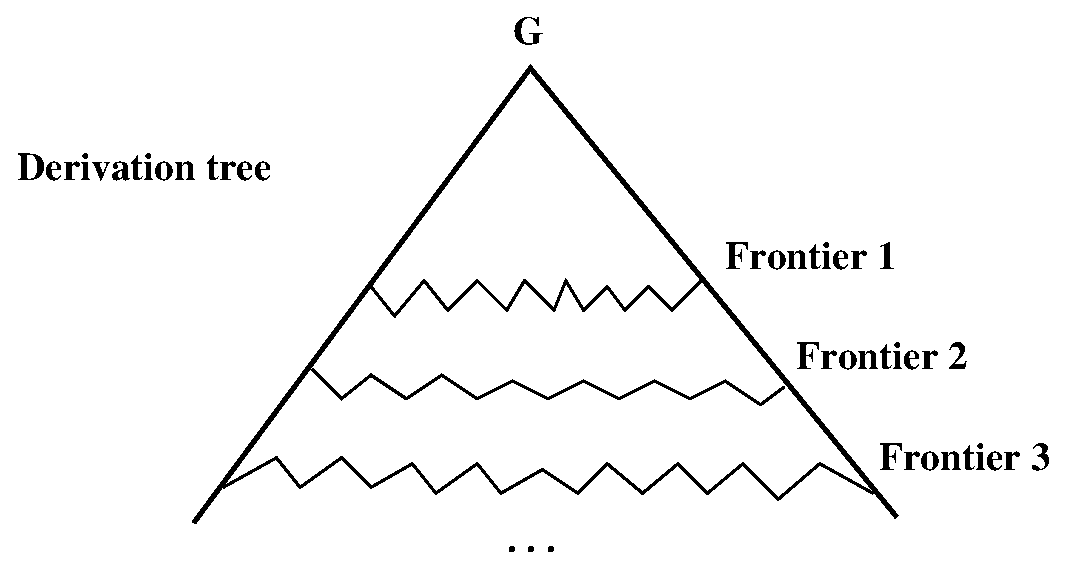
\includegraphics[width=4in]{tree_frontier.eps} 
        \caption{Frontiers of the goal $G$}
        \label{fig:tree_frontier}
  \end{figure}

In the figure \ref{fig:tree_frontier} there is a representation of different
frontiers in a derivation tree of a goal $G$. What is missing is a method to
generate the frontier. So far we have used the simplest possible frontier: the
frontier of depth 1 obtained by taking all the possible single SLD resolution
steps. This can be done by a simple inspection of the clauses of the
program.\footnote{Nevertheless, we plan to generate the frontier in a more
efficient way by using abstract interpretation over the input program for
detecting the degree of evaluation of a term that will be necesary at
execution time.} Additionally, built-in based goals receive a special
treatment (moving conjunctions into disjunctions, disjunctions into
conjunction, eliminating double negations, etc.)

\begin{definition}{\em Depth-one frontier}

    \begin{itemize} 

\item If $G \equiv (G_1;G_2) $ then $Frontier(G) \equiv$
$Frontier(G_1) \vee Frontier(G_2)$.

\item If $G \equiv (G_1,G_2) $ then $Frontier(G) \equiv$
  $Frontier(G_1) \wedge Frontier(G_2)$ and then we have to apply
  DeMorgan's distributive property to retain the disjunction
  of conjunctions format.
  
\item If $G \equiv p( \overline{X}) $ and 
  predicate $p/m$ is defined by N clauses: 

\begin{center}
\begin{tabular}{l}
$p( \overline{t}^1):- C_1 .$ \\
$\ldots$ \\
$p( \overline{t}^N):- C_N .$ \\
\end{tabular}
\end{center}

The frontier of the goal has the format: $Frontier(G) \equiv C_1
\vee C_2 \vee \ldots \vee C_N$, where each $C_i$ is the
conjunction of subgoals $C_i'$ and the equalities that are needed to
unify the variables of $\overline{X}$ (i.e. $C_i'~\wedge~\overline{X}
= \overline{t}^i$) and the respective terms of
$\overline{X}^i$.

    \end{itemize}

\end{definition}

The definition is an easy adaptation of Chan's one, but it is also a
simple example of the way we attack the problem, reformulating yet
defined concepts in an implementation oriented way.
\medskip

\noindent
Consider, for instance, the following code:
{
\begin{verbatim}
even(0).
even(s(s(X))) :- even(X).
\end{verbatim}
}
The frontier for the goal $even (Y)$ is as follows:

\[Frontier(even(Y)) = \{ ( Y=0 ) \vee ( Y=s(s(X)) \wedge even(X) ) \} \] 

  \begin{figure}
        \centering
        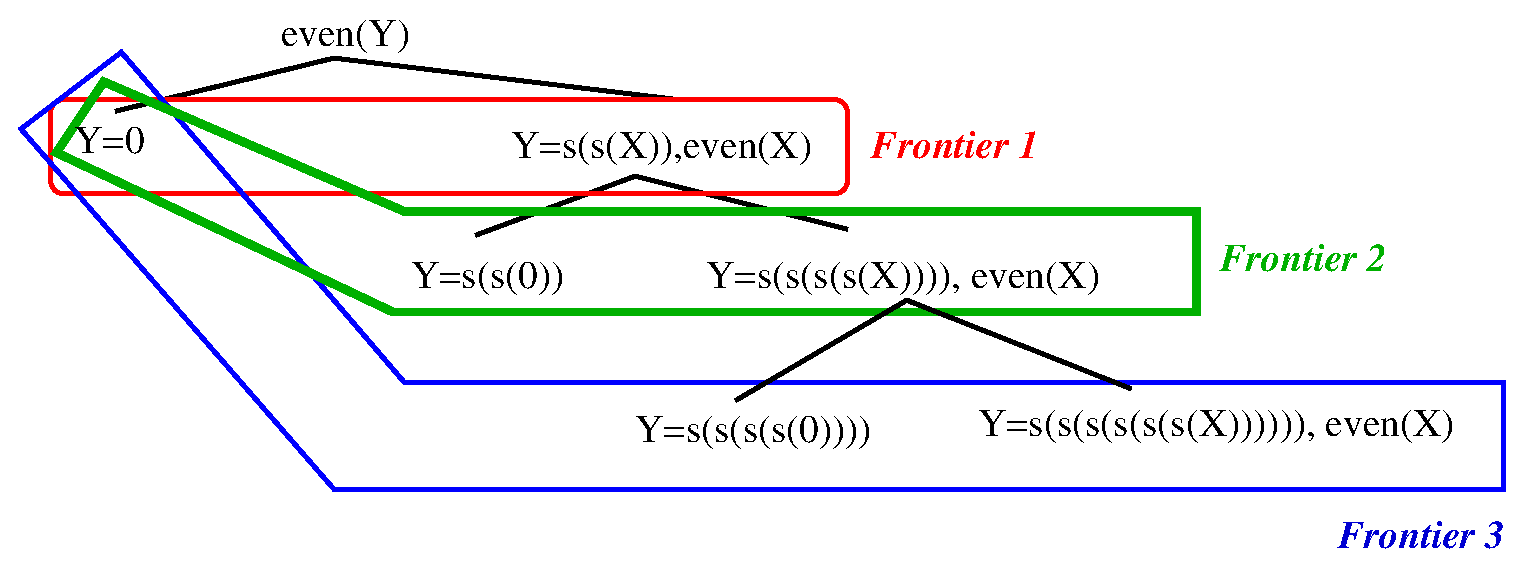
\includegraphics[width=5in]{frontier.eps} 
        \caption{First frontiers of the goal $even(Y)$}
        \label{fig:frontier}
  \end{figure}

Indeed, if we continue with the instantiation of the resolution tree we find
new frontiers more ``instantiated'' that are all equivalent to the initial
goal. See Figure~\ref{fig:frontier} where three frontiers of the goal
$even(Y)$ are represented.

Another example is:
{
\begin{verbatim}
parent(bob,mary).
parent(mary,joan).

grandparent(Y,X):- 
    parent(Y,Z),
    parent(Z,X).
\end{verbatim}
}

The frontier of the goal $grandparent (Y,X)$ has only one element in the
disjunction:
\[Frontier(grandparent(Y,X)) = \{ \exists Z (parent(Y,Z) \wedge parent(Z,X) ) \} \] 


\noindent
\implementation{A predicate $frontier/2$ has been
implemented. The call $frontier(G,Frontier)$ obtains the frontier (list of
lists of subgoals, i.e. disjunction of conjunctions of subgoals) of the goal
$G$. It is simple achieved by using the code expansion described in 
section \ref{expansion},
that provides predicates code at execution time.}

To get the negation of $G$ it suffices to negate the frontier
formula. This is done by negating each component of the disjunction of
all implied clauses (that form the frontier) and combining the
results. That is, $\neg ~ G \equiv \neg Frontier(G) \equiv \neg C~ _1
\wedge \ldots \wedge \neg~  C_N$.

Therefore, the solutions of $cneg(G)$ are the result of the
combination (conjunction) of one solution of each $\neg ~ C_i$. So, we
are going to explain how to negate a single conjunction $C_i$. This is
done in two phases: \emph{Preparation} and \emph{Negation of the
formula}.



%%%%%%%% PREPARATION %%%%%%%%%%%%%%%%%%%%%%%%%%%%%%%%%%%%%%
%\vspace{-0.1in}

\subsection{Preparation}
\label{preparation}

% Comparar con Chan

Before negating a conjunction obtained from the frontier, we have to
simplify, organize, and normalize this conjunction. The basic ideas are
present in \cite{Chan1} in a rather obscure way. In Chan's papers,
and then in Stuckey's one, it is simply stated that the conjunction is negated
using logic standard techniques. Of course, it is true but it is not so
easy in the middle of a Prolog computation because we have not
access to the whole formula or predicate we are executing.\footnote{unless 
we use metaprogramming techniques that we try to avoid for efficiency reasons}

\begin{itemize}

\item {\bf Simplification of the conjunction}. If one of the terms of
$C_i$ is trivially equivalent to $true$ (e.g. $X=X$), we can eliminate
this term from $C_i$. Symmetrically, if one of the terms is trivially
$fail$ (e.g. $X \neq X$), we can simplify $C_i \equiv fail$. The
simplification phase can be carried out during the generation of
frontier terms.

\item {\bf Organization of the conjunction}. Three groups are created
containing the components of $C_i$, which are divided into equalities
($\overline{I}$), disequalities ($\overline{D}$), and other subgoals
($\overline{R}$).  Then, we get $C_i \equiv \overline{I} \wedge
\overline{D} \wedge \overline{R}$. If we remember the examples that we have
provided for frontier:

$Frontier(even(Y)) = \{ C_1  \vee  C_2 \} = \{ ( Y=0 ) \vee ( Y=s(s(X)) \wedge
even(X) ) \}$ \\
$Frontier(grandparent(Y,X)) = \{ C_1'\} =   \{ \exists Z (parent(Y,Z) \wedge
parent(Z,X) )$ \\

We can organice the conjunctions $C_1, C_2$ and $C_1'$ following the division
into equalities, disequalities and rest as follow:\\
$C_1 \equiv ( Y=0 )  \wedge  \emptyset \wedge \emptyset$ \\
$C_2 \equiv  \exists X (~( Y=s(s(X)) ) \wedge \emptyset \wedge ( even(X) )~ )$ \\
$C_1' \equiv \exists Z (~ \emptyset \wedge \emptyset \wedge ( parent(Y,Z) \wedge
parent(Z,X)  ) ~)$ \\


\implementation{
We have provided a predicate $organization\_conj/5$ 
that receives in a call $organization\_conj(Conj,G,I,D,R)$ the conjuction
$Conj$ and the goal $G$. It returns in $I$ the values that are asigned to the
variables of $GoalVars$ in the equalities, in $D$ the list of the
disequalities and in $R$ the rest of subgoals of the conjunction
$Conj$. Arguments $I$, $D$ and $R$ are lists representing conjunctions of
equalities, disequalities and other subgoals repectively. The first argument
represents conjunctions using a pair $(Head,Body)$, where $Head$ is the
unification of the goal with the head of a clause (from where equalities, i.e.
unifications, can
be obtained), and $Body$ is the list that represents the conjunction of
subgoals of the body of a clause. 
In our example, in order to negate the  goal $even(Y)$, we call this predicate twice with
each of the two conjunctions of the frontier. 

First call: $organization\_conj((even(0),[]),even(Y),I,D,R)$ returns $I=[Y=0]$,
$D=[]$ and $R=[]$.

Second call: $organization\_conj((even(s(s(X))),[even(X)]),even(Y),I,D,R)$
returns $I=[Y=s(s(X))]$, $D=[]$, and $R=[even(X)]$.

To negate the goal $grandparent(Y,X)$, that is listed above, we call to \\
$organization\_conj((grandparent(A,B),[parent(A,C),parent(C,B)]),$ \\
$grandparent(Y,X),I,D,R)$,
returning $I=[X=B,Y=A]$, $D=[]$, and $R=[parent(A,C),parent(C,B)]$.

There are equalities when there are explicit unifications in the body of the
clauses or when there are implicit unifications in the head of the
clauses. Disequalities only appear if they are explicitly placed in the body of the
clauses.
}

\item {\bf Normalization of the conjunction}. Let us classify the variables in
the formula. The set of variables of the goal, $G$, is called $GoalVars$. The
set of free variables of $\overline{R}$ is called $RelVars$. We consider that
$ExpVars$ is the set of variables of $\overline{R}$ that are not in $ImpVars$,
i.e. $RelVars$, except the variables of $\overline{I}$ in the normalized
formula.

    \begin{itemize}

       \item {\bf Elimination of redundant variables and equalities}. If $I_i
       \equiv X = Y$, where $Y \not\in GoalVars$, then we now have the formula
       $ ( I_1 \wedge \ldots \wedge I_{i-1} \wedge I_{i+1} \wedge \ldots
       \wedge I_{NI} \wedge \overline{D} \wedge \overline{R}~) \sigma $, where
       $ \sigma = \{ Y / X \}$, i.e. the variable $Y$ is substituted by $X$ in
       the entire formula.
       \item {\bf Elimination of irrelevant disequalities}. $ImpVars$
       is the set of variables of $GoalVars$ and the variables that
       appear in $\overline{I}$. Disequalities $D_i$ that contain
       any variable that was neither in $ImpVars$ nor in $RelVars$ are
       irrelevant and should be eliminated.

    \end{itemize}

\implementation{
Before starting with the two steps of the
negation we should obtain the sets of variables that we will need for the
algorithm. We have implemented a predicate $normalization\_conj/9$ that in a
call  \linebreak
$normalization\_conj(I,D,R,GoalVars,In,Dn,Rn,ImpVars,ExpVars)$ receives
the equalities ($I$), disequalities ($D$), rest of subgoals ($R$) and list of variables of
$GoalVars$ and returns the updated equalities ($In$), disequalities ($Dn$) and rest of
subgoals ($Rn$ removing useless variables), and the sets of variables $ImpVars$ and
$ExpVars$.

In the example with $grandparent$ described above, the call \\
$normalization\_conj([X=B,Y=A], [], [parent(A,C),parent(C,B)], [Y,X],$ $ In, Dn,
Rn, ImpVars, ExpVars)$ 
returns $In=[]$, $Dn=[]$, $Rn=[parent(Y,C),$ $parent(C,X)]$, $ImpVars=[Y,X]$, and
$ExpVars=[C]$.
}
 \end{itemize}  
 

%%%%%%%% NEGATION OF THE FORMULA %%%%%%%%%%%%%%%%%%%%%%%%%%%%%%%%%
%\vspace{-0.1in}

\subsection{Negation of the formula}
\label{negation}

It is not feasible, to get all solutions of $C_i$ and to negate their
disjunction because $C_i$ can have an infinite number of solutions. So,
we have to use the classical constructive negation algorithm.

\medskip

\noindent
{\em First step: {\bf Division of the formula}}

\noindent
$C_i$ is divided into: 

\[~C_i \equiv \overline{I} \wedge
        \overline{D}_{imp} \wedge \overline{R}_{imp} \wedge
        \overline{D}_{exp} \wedge \overline{R}_{exp} \]

\noindent
where $\overline{D}_{exp}$ are the disequalities in $\overline{D}$
with variables in $ExpVars$ and $\overline{D}_{imp}$ are the other
disequalities, $\overline{R}_{exp}$ are the goals of $\overline{R}$
with variables in $ExpVars$ and $\overline{R}_{imp}$ are the other
goals, and $\overline{I}$ are the equalities.

If we consider for example one of the conjunctions of the frontier of
$even(Y)$ that is $C_2 \equiv ( Y=s(s(X)) ) \wedge \emptyset \wedge ( even(X)
)$ we can divide it into:

\begin{center}
\begin{tabular}{lllllllll}
$~~~~\overline{I}$ & $\wedge$ & 
        $\overline{D}_{imp}$ & $\wedge$ & $\overline{R}_{imp}$ & $
        \wedge$ &
        $\overline{D}_{exp}$ & $ \wedge$ & $ \overline{R}_{exp}$ \\
$\exists X (~ ( Y=s(s(X)) )$ & 
       $\wedge$ & $\emptyset$ & $ \wedge$ & $ (even(X))$ & $  \wedge$
        & $ \emptyset$ & $ \wedge$ & $\emptyset~)$ \\
\end{tabular}
\end{center}

Another example comes from the frontier of $parent(Y,X)$ that is the
conjunction $C_1' \equiv \emptyset \wedge \emptyset \wedge (\exists Z
(parent(Y,Z) \wedge parent(Z,X) )$ that can be divided into:
\begin{center}
\begin{tabular}{lllllllll}
$~~~~\overline{I}$ & $ \wedge$ &
        $\overline{D}_{imp}$ & $ \wedge$ & $ \overline{R}_{imp}$ &
        $\wedge$ & $\overline{D}_{exp}$ & $ \wedge$ & $ \overline{R}_{exp}$  \\
        $\exists Z (~ \emptyset$ & $ \wedge$ & $ \emptyset$ & $ \wedge$ & 
$\emptyset$ & $ \wedge$ & $ \emptyset$ & $ \wedge $ & $ (parent(Y,Z) \wedge parent(Z,X) ) ~)$ 
\end{tabular}
\end{center}


Therefore, the constructive negation of the divided formula is:

\noindent
$~~~~~~~~~~~~~~~~~~~~\neg~C_i \equiv \neg~\overline{I} \vee $ \\
$~~~~~~~~~~~~~~~~~~~~~~~~~~~~~~~~~~~~ ~~~~~~~~~~~~~~~~~~~~~~~~~~~~~~~~~~~(\overline{I} \wedge \neg~\overline{D}_{imp}) \vee  $ \\
$~~~~~~~~~~~~~~~~~~~~~~~~~~~~~~~~~~~~ ~~~~~~~~~~~~~~~~~~~~~~~~~~~~~~~~~~~(\overline{I} \wedge \overline{D}_{imp}  \wedge \neg~\overline{R}_{imp}) \vee $ \\
$~~~~~~~~~~~~~~~~~~~~~~~~~~~~~~~~~~~~ ~~~~~~~~~~~~~~~~~~~~~~~~~~~~~~~~~~~( \overline{I} \wedge \overline{D}_{imp} \wedge \overline{R}_{imp} \wedge \neg~(\overline{D}_{exp} \wedge \overline{R}_{exp})) $ \\

%% \noindent
%% \[ ~~~\neg~C_i \equiv \neg~\overline{I} \vee
%%  (\overline{I} \wedge
%% \neg~\overline{D}_{imp}) \vee 
%% (\overline{I} \wedge \overline{D}_{imp}
%% \wedge \neg~\overline{R}_{imp}) \vee
%% ( \overline{I} \wedge
%% \overline{D}_{imp} \wedge \overline{R}_{imp} \wedge
%% \neg~(\overline{D}_{exp} \wedge \overline{R}_{exp})) \]
%% \noindent

It is not possible to separate $\overline{D}_{exp}$ and
$\overline{R}_{exp}$ because they contain free variables and
they cannot be negated separately. The answers of the negations
will be the answers of the negation of the equalities, the answers of
the negation of the disequalities without free variables, the answers
of the negation of the subgoals without free variables and the answers
of the negation of the other subgoals of the conjunctions (the ones
with free variables). How to obtain each of this answers is described in the
second step.

\noindent
\emph{Implementation details}: We provide a predicate $divide\_formula/4$. A
call to the goal $divide\_formula(F,ExpVars,Fimp,Fexp)$ receives a formula $F$
that is a list of subgoals, and a list of variables $ExpVars$ and provide in
the lists of subgoals $Fimp$ all the subgoals from $F$ without any variable
from $ExpVars$ and in $Fexp$ the list with the rest of subgoals of $F$ (the
ones that contain any variable of $ExpVars$). This predicate is called twice:
 $divide\_formula(D,ExpVars,Dimp,Dexp)$, to split the set of disequalities
and, $divide\_formula(R,ExpVars,Rimp,Rexp)$, to split the set of the
rest of subgoals.

In the example of the negation of $even(Y)$, the first conjuction of the
frontier has empty sets $D$ and $R$. In the second conjunction $D$ is also 
empty, so the call $divide\_formula([],[],Dimp,Dexp)$ returns in both sets the
empty list. For the second conjunction the call
$divide\_formula([even(X)],[],Rimp,Rexp)$ returns $Rimp=[even(X)]$ and
$Rexp=[]$. Note that the set of free variables is empty.

In the example that negates $grandparent(Y,X)$, there are only one conjunction
and the first call to $divide\_formula([],[C],Dimp,Dexp)$ returns the empty
list in both variables. 

The second call $divide\_formula([parent(Y,C),parent(C,X)],[C],Rimp,Rexp)$
returns $Rimp=[]$ and $Rexp=[parent(Y,C),parent(C,X)]$.

These are simple examples, and although in general is less frecuent to find
non-empty disequalities sets, the regular case is a conjunction with free
variables, subgoals with them and subgoals without them (i.e. non empty sets
$Rimp$, $Rexp$). $\Box$
\medskip

\noindent
{\em Second step: {\bf Negation of subformulas}}

        \begin{itemize}

           \item {\bf Negation of $\overline{I}$}. We have $\overline{I}
           \equiv I_1 \wedge \ldots \wedge I_{NI} \equiv \exists~
           \overline{Z}_1~ X_1 = t_1 \wedge \ldots \wedge \exists~
           \overline{Z}_{NI}~ X_{NI} = t_{NI} $ where
           $\overline{Z}_i$ are the variables of the equality $I_i$ that
           are not included in $GoalVars$ (i.e. that are not quantified
           and therefore are free variables). When we negate this
           conjunction of equalities we get the constraint 
                $
           \underbrace{\forall~ \overline{Z}_1~ X_1 \neq t_1} _{\neg~
           I_1} \vee \ldots \vee \underbrace{\forall~
           \overline{Z}_{NI}~ X_{NI} \neq t_{NI} } _{\neg~ I_{NI}}
           \equiv %\] 
%                \[ 
           \bigvee_{i=1}^{NI} \forall~ \overline{Z}_i X_i
           \neq t_i $ 
           This constraint is the first answer of the negation of $C_i$ that
           contains $NI$ components.  In the example that we have seen that $
           I \equiv \exists X ~ Y=s(s(X))$, its negation is: $\overline{I}
           \equiv \forall~ X~~ Y \neq s(s(X))$.

\implementation{
The predicate $negate\_I/3$ implements this
task. The call to the goal $negate\_I(I,GoalVars,LSol)$ receives the list of
equalities and list of variables of $Goalvars$ and provides in $LSol$ the list
of solutions that represents the disjunction of the disequalities
obtained. There are as many solutions of the negation as elements in the
disjunction.   

During the negation of the set of equalities of the first conjunction of the
frontier of the goal $even(Y)$, the subgoal $negate\_I([Y=0],[Y],LSol)$ is
called and returns $LSol=[Y=/=0]$.
}

           \item {\bf Negation of $\overline{D}_{imp}$}. If we have
           $N_{D_{imp}}$ disequalities $\overline{D}_{imp} \equiv D_1
           \wedge \ldots \wedge D_{N_{D_{imp}}}$ where $ D_i \equiv
           \forall~ \overline{W}_i ~ \exists~ \overline{Z}_i ~~  Y_i
           \neq s_i$ where $Y_i$ is a variable of $ImpVars$, $s_i$ is
           a term without variables in $ExpVars$, $\overline{W}_i$ are
           universally quantified variables that are neither in the
           equalities \footnote{There are, of course, no universally
           quantified variables in an equality}, nor in the other
           goals of $\overline{R}$ because otherwise $\overline{R}$
           would be a disequality of $\overline{D}_{exp}$. Then we
           will get $N_{D_{imp}}$ new solutions with the format: 

           $~~~~~~~~~~~~~~~~~~~~\overline{I} \wedge \neg~ D_1 $ \\ 
           $~~~~~~~~~~~~~~~~~~~~\overline{I} \wedge
           D_1 \wedge \neg~ D_2 $ \\ 
           $~~~~~~~~~~~~~~~~~~~~\ldots $ \\ 
           $~~~~~~~~~~~~~~~~~~~~\overline{I} \wedge
           D_1 \wedge \ldots \wedge D_{N_{D_{imp}}-1} \wedge \neg~
           D_{N_{D_{imp}}}$ 

           where $ \neg~ D_i \equiv \exists~
           \overline{W}_i~ Y_i = s_i$. The negation of a universal
           quantification turns into an existential quantification and
           the quantification of free variables of $\overline{Z}_i$
           gets lost, because the variables are unified with the evaluation of
           the equalities of $\overline{I}$. Then, we will get
           $N_{D_{imp}}$ new answers.

\implementation{
The predicate $negate\_Dimp/2$ implements the
negation of these disequalities. Each call to $negate\_Dimp(Dimp,Sol)$
provides as many solutions in $Sol$ (as equalities) as disequalities there
are in $Dimp$. For example $negate\_Dimp([X=/=3,Y=/=5],Sol)$ returns two
answers with the solutions $X=3$ and $Y=5$. Indeed, solutions are returned
as lists of one only element for implementation reasons because to return the
complete solution of the negation, $SolC$, the negation of $Dimp$ should be
combined with the positive equalities (it is done by a simple
$append(I,Sol,SolC)$).
}

           \item {\bf Negation of $\overline{R}_{imp}$}. If we have
           $N_{R_{imp}}$ subgoals $\overline{R}_{imp} \equiv R_1 \wedge \ldots
           \wedge R_{N_{R_{imp}}}$. Then we will get new answers from each of
           the conjunctions:

           $~~~~~~~~~~~~~~~~~~~~\overline{I} \wedge \overline{D}_{imp} \wedge \neg~ R_1 $ \\ 
           $~~~~~~~~~~~~~~~~~~~~\overline{I} \wedge \overline{D}_{imp} \wedge
           R_1 \wedge \neg~ R_2 $ \\ 
           $~~~~~~~~~~~~~~~~~~~~\ldots $ \\ 
           $~~~~~~~~~~~~~~~~~~~~\overline{I} \wedge \overline{D}_{imp} \wedge
           R_1 \wedge \ldots \wedge R_{N_{R_{imp}}-1} \wedge \neg~
           R_{N_{R_{imp}}}$ 

           where $ \neg~ R_i \equiv cneg(R_i)$. Constructive negation is
           applied over $R_i$ recursively.
           In the example of $C_2$ from the frontier of $even(Y)$ we will
           provide the answer: $Y = s(s(X)) \wedge \neg~even(X)$.

\implementation{
The predicate $negate\_Rimp/2$ provides the
negation of the subgoals of $Rimp$. For example, in the negation of the second
conjunction of the frontier of $even(Y)$, from the call
$negate\_Rimp([even(X)],Sol)$ the solution $cneg(even(X))$ is obtained
that later is combined with the positive equalities and disequialities, and the
solution $[Y=s(s(X)),cneg(even(X))]$ is provided. Before returning the answer,
all its subgoals are combined and in this case the new execution of $cneg$
will provide results that will be combined with the equality. The backtracking
will give as many answers (going deeper and deeper in the recursive calls)
as we want.
}

           \item {\bf Negation of $\overline{D}_{exp} \wedge
           \overline{R}_{exp}$}. This conjunction cannot be separated
           because of the negation of $ \exists~ \overline{V}_{exp}~
           \overline{D}_{exp} \wedge \overline{R}_{exp}$, where
           $\overline{V}_{exp}$ gives universal quantifications:\\
           $\forall~ \overline{V}_{exp}~ cneg(\overline{D}_{exp}
           \wedge \overline{R}_{exp})$. The entire constructive
           negation algorithm must be applied again. Notice the
           recursive application of constructive negation. However,
           the previous steps could have generated an answer for the
           original negated goal. Of course it is possible to produce
           infinitely many answer to a negated goal.

           Note that the new set $GoalVars$ is the former set
           $ImpVars$. Variables of $\overline{V}_{exp}$ are considered
           as free variables. When solutions of
           $cneg(\overline{D}_{exp} \wedge \overline{R}_{exp})$ are
           obtained some can be rejected: solutions with equalities
           with variables in $\overline{V}_{exp}$. If there is a
           disequality with any of these variables, e.g. $V$, the
           variable will be universally quantified in the disequality.
           This is the way to obtain the negation of a goal, but there
           is a detail that was not considered in former approaches
           and that is necessary to get a sound implementation: the
           existence of universally quantified variables in
           $\overline{D}_{exp} \wedge \overline{R}_{exp}$ by the
           iterative application of the method. That is, we are really
           negating a subgoal of the form: $ \exists~~
           \overline{V}_{exp}~ \overline{D}_{exp} \wedge
           \overline{R}_{exp}$. Its negation is $\forall~
           \overline{V}_{exp}~~ \neg(\overline{D}_{exp} \wedge
           \overline{R}_{exp})$ and therefore, we will provide the
           last group of answers that comes from:

           \[\overline{I} \wedge \overline{D}_{imp}
           \wedge \overline{R}_{imp} \wedge \forall~
           \overline{V}_{exp}~ \neg~(\overline{D}_{exp} \wedge
           \overline{R}_{exp})\]

	   In the conjunction $C_1'$ from the frontier of $grandparent(Y,X)$
           we obtain the answer: $\forall~ Z ~ \neg~(parent(Y,Z) \wedge
           parent(Z,X))$.

\implementation{
We have implemented 
$negate\_Dexp\_Rexp/3$. A call to
$negate\_Dexp\_Rexp(DRexp,ImpVars,ExpVars,Sol)$ receives the set of
disequalities and the rest of subgoals with free variables, $DRexp$, the list
of variables of the equalities, $ImpVars$, and the list of free variables
$ExpVars$. It returns a solution $Sol$ that is the negation of the conjunction
of subgoals of $DRexp$.  In the example of negating $grandfather(Y,X)$, the
call to $negate\_Dexp\_Rexp([parent(Y,C),parent(C,X)],[Y,X],[C],Sol)$ returns
the single list,
$Sol=[cneg\_aux((parent(Y,C),parent2(C,X)),[Y,X],[C])]$. The predicate
$cneg\_aux/3$ is equivalent to the constructive negation, $cneg/1$, but with
two additional arguments, $cneg\_aux(Goal,GoalVars,UnivVars)$, that are the
list of existencial variables of the goal that is going to be negated and the
list of the universal variables (that comes from the negation of the free
variables). This detail of taking into account the universal variables in the
recursive calls to the negation is one of the keys to achieve a real
constructive implementation. It is also necessary to joint to this solution
the equalities and disequalities without free variables before providing an
answer, with a call $append(I\_Dimp\_Rimp,Sol,SolC)$.
}

         \end{itemize}


    

%%%%%%%%%%%%%%%%%%%%%%%%%%%%%%%%%%%%%%%%%%%%%%%%%%%%%%%%%%%%%%%%%%
%%%%%%%%%%%%%%%  IMPLEMENTATION ISSUES  %%%%%%%%%%%%%%%%%%%%%%%%%%
%%%%%%%%%%%%%%%%%%%%%%%%%%%%%%%%%%%%%%%%%%%%%%%%%%%%%%%%%%%%%%%%%%

\section{Implementation Issues}
\label{implementation}

Having described the theoretical algorithm, including important
details, we now discuss important aspects for a practical
implementation, including how to compute the frontier and manage
answer constraints.

%%%%%%%% CODE EXPANSION  %%%%%%%%%%%%%%%%%%%%%%%%%%%%%%%%%

%\vspace{-0.1in}
\subsection{Code Expansion}
\label{expansion}

The first issue is how to get the frontier of a goal. It is possible to handle
the code of clauses during the execution thanks to the Ciao package system
\cite{ciao-modules-cl2000}, which allows the code to be expanded at run
time. The expansion is implemented in the $cneg$.pl package which is included
in the declaration of the module that is going to be expanded (i.e. where
there are goals including negation). The loading of the $cneg$.pl package
means that the compiler works with an expanded code added to the previous
code. For each clause, $H~:-~B_1,...,B_n$, of the input program, a new fact
$stored\_clause(H,[B_1,...,B_n])$ is added.

Consider a module $even$ where the predicate $even/1$ and its negation are
defined: 

\begin{verbatim}
:- module(even,[even/1,not_even/1],[cneg]).

even(0).
even(s(s(X))) :- even(X).

not_even(X) :- cneg(even(X)).
\end{verbatim}

At compilation time this input program is expanded with these two new facts of
the predicate $stored\_clause/2$:  

\begin{verbatim}
stored_clause(even(0),[]).
stored_clause(even(s(s(X))),[even(X)]).
\end{verbatim}

\noindent
where information about code structure is stored to be used by the negation
algorithm. Now, the execution is able to compute the frontier we described
above $\{ ( Y=0 ) \vee ( Y=s(s(X)) \wedge even(X) ) \}$

Note that a similar, but less efficient, behaviour can be emulated
using metaprogramming facilities, available in most Prolog compilers.
 

%%%%%%%% DISEQUALITY CONSTRAINTS  %%%%%%%%%%%%%%%%%%%%%%%%%%%%%%%%%
%\vspace{-0.1in}
\subsection{Disequality constraints}
\label{disequality}

An instrumental step for managing negation is to be able to handle
disequalities between terms such as $t_1 \neq t_2$.  The typical
Prolog resources for handling these disequalities are limited to the
built-in predicate {\tt /== /2}, which needs both terms to be ground
because it always succeeds in the presence of free variables.  It is
clear that a variable needs to be bound with a disequality to achieve
a ``constructive'' behaviour.  Moreover, when an equation $X =
t(\overline{Y})$ is negated, the free variables in the equation must
be universally quantified, unless affected by a more external
quantification, i.e. $\forall~ \overline{Y}~X \neq t(\overline{Y})$ is
the correct negation.  As we explained in \cite{SusanaPADL2000}, the
inclusion of disequalities and constrained answers has a very low
cost. From the theoretical point of view, it incorporates negative normal form 
constraints (in the form of conjuntion of equalities plus conjunction of 
disjunctions of possibly universally quantified
disequations) instead of simple bindings as the decomposition step can produce 
disjunctions. In the implementation side, attributed variables are used 
which associate a data structure, containing a
normal form constraint, to any variable: 

\[~~~~( \underbrace{\bigwedge_j \forall~ \overline{Z}_j^1~(Y_j^1 \neq s_j^1) 
\vee \ldots \vee \bigwedge_l \forall~ \overline{Z_l}^n~(Y_l^n \neq s_l^n) ) }_{\mbox{negative information}} \]
%% %\vspace{-20pt}

%% \noindent
%% where each $X_i$ appears only in $X_i = t_i$, no $s_k^r$ is $Y_k^r$
%% and the universal quantification could be empty (leaving a simple
%% disequality).

%% It is easy to see that some normalization rules can be defined for a
%% normal form formula from any initial formula. The redefinition of the
%% unification algorithm to manage constrained variables is also a simple
%% exercise.

%% \cite{Moreno1} introduces this very compact way to represent a normal
%% form constraint.  Chan's representation uses only disjunctions and
%% they are dealt with by means of backtracking. The main advantage of our
%% normal form is that the search space is drastically reduced.

%% To include disequalities into a Prolog compiler, we need to just
%% reprogram unification. This can be done using attributed variables
%% \cite{Carlsson} (available in several Prolog versions, e.g. in Sicstus
%% Prolog, or in Eclipse, where they are called meta-structures). These
%% variables allow us to keep information associated with each variable
%% (in an attibute that is a term) during the unification, which can be
%% used to dynamically control the constraints.

%% %% Attributed variables are variables with an associated attribute.  which
%% %% is a term. Each variable has an associated data structure, containing a
%% %% normal form constraint: a list of lists of pairs (variable, term). They
%% %% behave like ordinary variables, except that the programmer can supply
%% %% code for unification, printing facilities and memory management. In
%% %% our case, the printing facility is used to show constrained
%% %% answers. The main task is to provide a new unification code.

%% For the unification of a variable $X$ with a term $t$, there are three
%% possible cases (up to commutativity):

%% %\vspace{-5pt}
%% \begin{enumerate}
%% %\addtolength{\itemsep}{-8pt}

%%    \item $X$ is a free variable and $t$ is not a variable with a
%%    negative constraint: just bind $X$ to $t$,

%%    \item $X$ is a free variable or bound to a term $t'$ and $t$ is a
%%    variable $Y$ with a negative constraint: check whether $X$ (or,
%%    equivalently, $t'$) satisfies the constraint associated with $Y$.
%%    A conveniently defined predicate {\tt satisfy} is used for this
%%    purpose,

%%    \item $X$ is bound to a term $t'$ and $t$ is a term (or a variable
%%    bound to a term): use the classical unification algorithm.

%% \end{enumerate}
%% %\vspace{-5pt}

Additionaly, a Prolog predicate {\tt =/= /2} has been defined, used to
check disequalities, similarly to explicit unification ({\tt =}). Each
constraint is a disjunction of conjunctions of disequalities. A
universal quantification in a disequality (e.g., $\forall Y~ X \neq
c(Y)$), is represented with a new constructor {\tt fA}$/1$ (e.g., {\tt
X =/= c(fA(Y)))}.  We refer the interested
reader to check the details in \cite{SusanaPADL2000}.

%% The first list is used to represent
%% disjunctions while the internal list represents the conjunction of
%% disequalities.

Let us show some examples involving variable $X$ where we show the
corresponding attribute that represents the constraint of each
subgoal\footnote{The predicate forall/2 implements the universal
quantification. I.e. $forall(L,E)$ quantify universally the set of variables
$L$ in the expression $E$}: 

%\hspace{-0.5cm}
\begin{center}
\begin{small}
\begin{tabular}{lll}
SUBGOAL & ATTRIBUTE & CONSTRAINT \\
\hline\hline
\ \\
{\tt not\_member(X,[1,2,3])}   &  $X=/=1,X=/=2,X=/=3$  & $X \neq 1 \wedge X \neq 2 \wedge X \neq 3$\\
{\tt member(X,[1,2,3]),X=/=2}  &  $X=/=1,X=/=3$        & $X \neq 1 \wedge X \neq 3$\\
{\tt member(X,[1]), X=/=1}     &  {\tt fail}           & $false$ \\
{\tt X =/= 4}                  & $X=/=4$               & $X \neq 4$ \\
{\tt X =/= 4; X=/=5}           & $X=/=4~ ;~ X/5$       & $X \neq 4 \vee X \neq 5$ \\
{\tt X =/= 5; (X=/=6, X=/=Y)}  & $X=/=5 ~;                 $    & $X \neq 5 \vee                           $\\
                               & $           (X=/=6, X=/=Y)$    & $              (X \neq 6 \wedge X \neq Y)$\\
{\tt forall([Y], X =/= s(Y))}  & $X=/=s(fA(Y)$         & $\forall Y. X \neq Y$ \\
%{\tt (member (X,[0,s(0),s(s(0))]),} &                  & \\
%{\tt forall (Y, X =/= s (Y)) )}     & $0$              & $X = 0$
\end{tabular}
\end{small}
\end{center}



%%%%%%%% OPTIMIZATION  %%%%%%%%%%%%%%%%%%%%%%%%%%%%%%%%%
%\vspace{-0.1in}

\subsection{Optimizing the algorithm and the implementation}
\label{optimization}

Our constructive negation algorithm and the implementation techniques
admit some additional optimizations that can improve the runtime
behaviour of the system. Basically, the optimizations rely on the
compact representation of information, as well as the early detection
of successful or failing branches.
\bigskip

\noindent
{\bf Compact information}. In our system, negative information is
represented quite compactly thanks to our constraint normal form,
providing fewer solutions from the negation of $\overline{I}$ and
$\overline{D}_{imp}$. The advantage is twofold. On the one hand
constraints contain more information and failing branches can be
detected earlier (i.e. the search space could be smaller). On the
other hand, if we ask for all solutions using backtracking, we are
cutting the search tree by offering all the solutions together in a
single answer. For example, we can offer a simple answer for the
negation of a predicate $p$ (the code for $p$ is skipped because it is
no relevant for the example): {
\begin{verbatim}
?- cneg(p(X,Y,Z,W)).
(X=/=0, Y=/=s(Z)) ; (X=/=Y) ; (X=/=Z) ; 
(X=/=W) ; (X=/=s(0), Z=/=0) ? ;
no
\end{verbatim}
}
\noindent
(which is equivalent to the formula $ (X \neq 0 \wedge Y\neq s(Z))
\vee X \neq Y \vee X \neq Z \vee X \neq W \vee (X \neq s(0) \wedge Z
\neq 0)$ that can be represented in our constraint normal form and,
therefore, managed by attributes to the involved variables), instead
of returning the six equivalent answers upon backtracking: {
\begin{verbatim}
?- cneg(p(X,Y,Z,W)).
X=/=0, Y=/=s(Z) ? ;
X=/=Y ? ;
X=/=Z ? ;
X=/=W ? ;
X=/=s(0), Z=/=0 ? ;
no
\end{verbatim}
} 
\noindent
In this case we get the whole disjunction at once instead of getting
it by backtraking step by step. The generation of compact formulas in
the negation of subformulas (see above Second step) is used whenever
possible (in the negation of $\overline{I}$ and the negation of
$\overline{D}_{imp}$). The negation of $\overline{R}_{imp}$ and the
negation of $(\overline{D}_{exp} ~ \vee ~ \overline{R}_{exp})$ can
have infinite solutions whose disjunction would be impossible to
compute. So, for these cases we construct incrementally the solutions
using backtracking.
\bigskip

\noindent
{\bf Pruning subgoals}. The frontier generation search tree can be
cut with a double action over the ground subgoals: removing the
subgoals whose failure we are able to detect early on, and simplifying the
subgoals that can be reduced to true. Suppose  we have a predicate $p/2$
defined by
{
\begin{verbatim}
p(X,Y):- greater(X,Y), q(X,Y,Z), r(Z).
\end{verbatim}
}\noindent
where $q/3$ and $r/1$ are predicates defined by several
clauses with a complex computation. To negate
the goal $p(s(0),s(s(0)))$, its frontier is computed:

$~~~~~~~~~~~~~~~~~Frontier(p(s(0),s(s(0)))) \equiv $ \\
$Step~ 1~~~~~~~~~~~~{ X=s(0) \wedge Y=s(s(0)) \wedge
  greater(X,Y) \wedge q(X,Y,Z) \wedge r(Z) } \equiv $ \\
$Step~ 2~~~~~~~~~~~~{ greater(s(0),s(s(0))) \wedge q(s(0),s(s(0)),Z) \wedge r(Z) } \equiv $ \\
$Step~ 3~~~~~~~~~~~~{ fail  \wedge q(s(0),s(s(0)),Z) \wedge r(Z) } \equiv $ \\
$Step~ 4~~~~~~~~~~~~fail $ \\

The first step is to expand the code of the subgoals of the frontier
to the combination of the code of all their clauses (disjunction of
conjunctions in general but only one conjunction in this case because
$p/2$ is defined by only one clause), and the result will be a very
complicated and hard to check frontier.  However, the process is
optimized by evaluating ground terms (Step 2). In this case,
$greater(s(0),s(s(0))$ fails and, therefore, it is not necessary to
continue with the generation of the frontier, because the result is
reduced to fail (i.e. the negation of $p (s(0), s(s(0)))$ will be
trivially true). The opposite example is a simplification of a
successful term in the third step:

$~~~~~~~~~~~~~~~~~Frontier(p(s(s(0)),s(0))) \equiv $\\
$Step~ 1~~~~~~~~~~~~{ X=s(s(0)) \wedge Y=s(0) \wedge greater(X,Y) \wedge q(X,Y,Z) \wedge
  r(Z) } \equiv $ \\
$Step~ 2~~~~~~~~~~~~{ greater(s(s(0)),s(0)) \wedge q(s(s(0)),s(0),Z) \wedge r(Z) } \equiv
$ \\
$Step~ 3~~~~~~~~~~~~{ true \wedge q(s(s(0)),s(0),Z) \wedge r(Z) } \equiv $ \\
$Step~ 4~~~~~~~~~~~~{ q(s(s(0)),s(0),Z) \wedge r(Z) } $ \\

\noindent
{\bf Constraint simplification}. During the whole process for negating
a goal,the frontier variables are constrained. In cases where the
constraints are satisfiable, they can be eliminated and where the
constraints can be reduced to fail, the evaluation can be stopped with
result \emph{true}.
 
We focus on the negative information of a normal form constraint $F$:

$~~~~~~~~~~~~~~~~~ F \equiv  \bigvee_i\bigwedge_j \forall~ \overline{Z}_j^i~(Y_j^i \neq s_j^i)$

Firstly, the Prenex form \cite{Shoenfield} can be obtained by
extracting the universal variables with different names to the head of
the formula, applying logic rules:

$~~~~~~~~~~~~~~~~~ F \equiv \forall \overline{x} \bigvee_i\bigwedge_j (Y_j^i \neq s_j^i) $

\noindent
and using the distributive property (notice that subindexes are different):

$~~~~~~~~~~~~~~~~~ F \equiv \forall \overline{x} \bigwedge_k\bigvee_l (Y_l^k \neq s_l^k) $

The formula can be separated into subformulas that are simple
disjunctions of disequalities :

 $~~~~~~~~~~~~~~~~~ F \equiv \bigwedge_k \forall \overline{x} \bigvee_l (Y_l^k \neq s_l^k) \equiv F_1 \wedge ... \wedge F_n$

Each single formula $F_k$ can be evaluated. The first step will be to
substitute the existentially quantified variables (variables that do not
belong to $\overline{x}$) by Skolem constants that will keep
the equivalence without losing generality:

$~~~~~~~~~~~~~~~~~  F_k \equiv \forall \overline{x} \bigvee_l ( Y_l^k \neq s_l^k ) \equiv \forall \overline{x} \bigvee_l ( Y_{Sk l}^k \neq s_{Sk l}^k )  $

Then it can be transformed into:

$~~~~~~~~~~~~~~~~~ F_k \equiv  \neg \exists ~ \overline{x} \neg ( \bigvee_l (Y_{Sk l}^k \neq s_{Sk l}^k) ) \equiv \neg Fe_K $

The meaning of $F_k$ is the negation of the meaning of $Fe_k$;

$~~~~~~~~~~~~~~~~~ Fe_k \equiv \exists ~ \overline{x} \neg ( \bigvee_l (Y_{Sk l}^k \neq s_{Sk l}^k)) $
 
Solving the negations, the result is obtained through simple unifications of the variables of $\overline{x}$:

$~~~~~~~~~~~~~~~~~  Fe_k  \equiv \exists ~ \overline{x} \bigwedge \neg (Y_{Sk l}^k \neq s_{Sk l}^k)  \equiv \exists ~ \overline{x} \bigwedge (Y_{Sk l}^k = s_{Sk l}^k)  $

        Therefore, we get the truth value of $F_k$ from the
        negation of the value of $Fe_k$ and, finally, the value of $F$ is
        the conjunction of the values of all $F_k$. If $F$
        succeeds, then the constraint is removed because it is redundant
        and we continue with the negation process. If it fails, then
        the negation directly succeeds.

%%%%%%%%%%%%%%%%%%%%%%%% RESULTS %%%%%%%%%%%%%%%%%%%%%%%%%%%%%%%%%

\section{Experimental results}
\label{results}

Our prototype is a simple library that is added to the set of
libraries of Ciao Prolog. Indeed, it is easy to port the library to
other Prolog compilers. The only requirement is that attributed
variables should be available.

This section reports some experimental results from our prototype
implementation.  First of all, we show the behaviour of the
implementation in some simple examples.

%%%%%%%% EXAMPLES  %%%%%%%%%%%%%%%%%%%%%%%%%%%%%%%%%
%\vspace{-0.1in}

\subsection{Examples}
\label{examples}

The interesting side of this implementation is that it returns
constructive results from a negative question. Let us start with a
simple example involving predicate $boole/1$.

{
\begin{minipage}{2in}
\begin{verbatim}
boole(0).
boole(1).
\end{verbatim}
\end{minipage}
\begin{minipage}{2in}
%\rnode{A}{}
\begin{verbatim} 

    ?- cneg(boole(X)).
    X=/=1, X=/=0 ? ;
    no

\end{verbatim} 
%\rnode{B}{}
%\ncline{A}{B}
\end{minipage}\\
}
Another simple example obtained from \cite{Stuckey95} gives us the
following answers:

{
\begin{minipage}{2in}
\begin{verbatim}
p(a,b,c).
p(b,a,c).
p(c,a,b).
proof1(X,Y,Z):-
    X =/= a, Z = c,
    cneg(p(X,Y,Z)).

\end{verbatim}
\end{minipage}
\begin{minipage}{2in}
\begin{verbatim} 
   ?- proof1(X,Y,Z).
   Z = c, X=/=b, X=/=a ? ;
   Z = c, Y=/=a, X=/=a ? ;
   no
\end{verbatim} 
\end{minipage}\\
}
\cite{Stuckey95} contains another example showing how a constructive
answer ($\forall T ~ X \neq s(T)$) is provided for the negation of an
undefined goal in Prolog:

{
\begin{minipage}{2in}
\begin{verbatim}

p(X):- X = s(T), q(T).
q(T):- q(T).
r(X):- cneg(p(X)).
\end{verbatim}
\end{minipage}
\begin{minipage}{2in}
\begin{verbatim} 
   ?- r(X).
   X=/=s(fA(_A)) ?
   yes
\end{verbatim} 
\end{minipage}\\
}


Notice that if we would ask for a second answer, then it will loop
according to the Prolog resolution. An example with an infinite number
of solutions is more interesting.

{
\begin{minipage}{1.5in}
\begin{verbatim}
positive(0). 
positive(s(X)):-
        positive(X).  
\end{verbatim}
\end{minipage} 
\begin{minipage}{2.5in}
%\rnode{A}{}
\begin{verbatim} 

    ?- cneg(positive(X)).
    X=/=s(fA(_A)), X=/=0 ? ;
    X = s(_A), 
    (_A=/=s(fA(_B)), _A=/=0) ? ;
    X = s(s(_A)), 
    (_A=/=s(fA(_B)), _A=/=0) ? ;
    X = s(s(s(_A))),
    (_A=/=s(fA(_B)), _A=/=0) ? 
    yes
\end{verbatim} 
%\rnode{B}{}
%\ncline{A}{B}
\end{minipage}
}
%% \begin{minipage}{1.5in}
%% \begin{verbatim}
%% number(0).
%% number(s(X)):-
%%         number(X).

%% greater(s(X),0):-
%%         number(X).
%% greater(s(X),s(Y)):-
%%         greater(X,Y).
%% \end{verbatim}
%% \end{minipage}
%% \begin{minipage}{2.5in}
%% %\rnode{A}{}
%% \begin{verbatim} 
%%     ?- cneg(greater(X,Y)).

%%     Y=/=0, Y=/=s(fA(_A)) ? ;

%%     (Y=/=s(fA(_A))), 
%%     (X=/=s(fA(_B))) ? ;

%%     X = s(_A),Y = 0,
%%     (_A=/=s(fA(_B)),_A=/=0) ? ;

%%     X = s(s(_A)),Y = 0,
%%     (_A=/=s(fA(_B)),_A=/=0) ? ;

%%     X = s(s(s(_A))),Y = 0,
%%     (_A=/=s(fA(_B)),_A=/=0) ? ;

%%     X = s(s(s(s(_A)))),Y = 0,
%%     (_A=/=s(fA(_B)),_A=/=0) ? 

%%     yes
%% \end{verbatim} 
%% %\rnode{B}{}
%% %\ncline{A}{B}
%% \end{minipage}
%\vspace{-0.1in}

\subsection{Implementation measures}

We have firstly measured the execution times in milliseconds for the
above examples when using negation as failure ($naf/1$) and
constructive negation ($cneg/1$). A `-' in a cell means that negation
as failure is not applicable. Some goals were executed a number of
times to get a significant measurement. All of them were made using
\ciao\ Prolog\footnote{The negation system is coded as a library
module (``package'' \cite{ciao-modules-cl2000}), which includes the
respective syntactic and semantic extensions (i.e. Ciao's attributed
variables). Such extensions apply locally within each module which
uses this negation library.} 1.5 on a Pentium II at 350 MHz. The
results are shown in Table~\ref{table}. We have added a first column
with the runtime of the evaluation of the positive goal that is
negated in the other columns and a last column with the ratio that
measures the speedup of the \naf\ technique w.r.t. constructive
negation.

Using {\bf naf} instead of {\bf cneg} results in small ratios around
1.06 on average for ground calls with few recursive calls. So, the
possible slow-down for constructive negation is not so high as we
might expect for these examples. Furthermore, the results are rather
similar. But the same goals with data that involve many recursive
calls yield ratios near 14.69 on average w.r.t {\bf naf},
increasing exponentially with the number of recursive calls. There
are, of course, many goals that cannot be negated using the \naf\
technique and that are solved using constructive negation.

\begin{table}[t]
%\begin{small} 
\begin{tabular}{||l|r|r|r|r||}
\hline %------------------------------------------------------------------
\hline %-------------------------------------------------------------------
{\bf goals} &~~ {\bf Goal} ~~& ~~{\bf naf(Goal) }~~ &~~ {\bf cneg(Goal)}~~ &~~ {\bf ratio}~~ \\ 

\hline %--------------------------------------------------
boole(1)                     &  2049      &  2099    &  2069   &   0.98   \\ 
\hline %--------------------------------------------------
boole(8)                     &  2070      &  2170    &  2590   &   1.19   \\ 
\hline %--------------------------------------------------
boole(X)                     &  2080      &  -       &  3109   &          \\ 
\hline %--------------------------------------------------
positive(s(s(s(s(s(s(0))))))~~~ &  2079      &  1600    &  2159   &   1.3    \\ 
\hline %--------------------------------------------------
positive(s(s(s(s(s(0))))))   &  2079      &  2139    &  2060   &   0.96   \\ 
\hline %--------------------------------------------------
positive(X)                  &  2020      &  -       &  7189   &          \\ 
\hline %--------------------------------------------------
greater(s(s(s(0))),s(0))     &  2110      &  2099    &  2100   &   1.00   \\ 
\hline %--------------------------------------------------
greater(s(0),s(s(s(0))))     &  2119      &  2129    &  2089   &   0.98   \\ 
\hline %--------------------------------------------------
greater(s(s(s(0))),X)        &  2099      &  -       &  6990   &          \\ 
\hline %--------------------------------------------------
greater(X,Y)                 &  7040      &  -       &  7519   &          \\ 
\hline %--------------------------------------------------
queens(s(s(0)),Qs)           &  6939      &  -       &  9119   &          \\ 

\hline %-------------------------------------------------------
\hline %-------------------------------------------------------
{\bf average}                &            &          &         &   1.06   \\ 
\hline %--------------------------------------------------------------------------------
\hline %--------------------------------------------------------------------------------
\end{tabular}
\vspace*{3mm}
\caption{Runtime comparation}
\label{table}
%\end{small}
\end{table}
 
 

%%%%%%%%%%%%%%%%%%%%%%%%%%%%%%%%%%%%%%%%%%%%%%%%%%%%%%%%%%%%%%%%%%
%%%%%%%%%%% FINITE CONSTRUCTIVE NEGATION  %%%%%%%%%%%%%%%%%%%%%%%%
%%%%%%%%%%%%%%%%%%%%%%%%%%%%%%%%%%%%%%%%%%%%%%%%%%%%%%%%%%%%%%%%%%

\section{Finite Constructive Negation}
\label{cnegf}

The problem with the constructive negation algorithm is of course
efficiency. It is the price that it has to be paid for a powerful
mechanism that negates any kind of goal. Thinking of Prolog programs,
many goals have a finite number of solutions (we are considering also
that this can be discovered in finite time, of course). There is a
simplification of the constructive negation algorithm that we use to
negate these goals. It is very simple in the sense that if we have a
goal $\neg G$ where the solution of the positive subgoal $G$ is a set
of $n$ solutions like $\{S_1, S_2,...,S_n\}$, then we can consider
these equivalences: %%$$~~~~G \equiv S_1 \vee S_2 \vee ... \vee S_n $$
$~~~~~~~~\neg G \equiv \neg(S_1 \vee S_2 \vee ... \vee S_n) 
 \equiv (\neg S_1 \wedge \neg S_2 \wedge ... \wedge \neg S_n)$

Of course, these solutions are a conjunction of unifications
(equalities) and disequality constraints. As described in section
\ref{disequality}, we know how to handle and negate this kind of
information. The implementation of the predicate $cnegf/1$ is
something akin to

{
\begin{verbatim}
cnegf(Goal):-
  varset(Goal,GVars), % Getting variables of the Goal
  setof(GVars,Goal,LValores),!, % Getting the solutions
  cneg_solutions(GVars,LValores). % Negating solutions
cnegf(_Goal). % Without solutions, the negation succeeds
\end{verbatim}
}
\noindent
where $cneg\_solutions/2$ is the predicate that negates the disjunction
of conjunctions of solutions of the goal that we are negating. It
works as described in section \ref{negation}, but it is simpler,
because here we are only negating equalities and disequalities.

We get the set of variables, $GVars$, of the goal, $Goal$, that we
want to negate (we use the predicate $varset/2$). Then we use the
$setof/3$ predicate to get the values of the variables of $GVars$
 for each solution of $Goal$. For example, if we want to
evaluate $cnegf(boole(X))$, then we get $varset(boole(X),[X])$,
$setof([X],boole(X),[[0],[1]])$ (i.e. $X=0 \vee X=1$) and
$cneg\_solutions/2$ will return $X \neq 0
\wedge X \neq 1$. 

If we have the goal $p(X,Y)$, which, has two solutions $X=a,~Y=b$ and
$X=c,~Y=d$, then, in the evaluation of $cnegf(p(X,Y))$, we will get
$varset(p(X,Y),$ $[X,Y])$, $setof([X,Y],p(X,Y),[[a,b],[c,d]])$
(i.e. $(X=a \wedge Y=b) \vee (X=c \wedge Y=d)$) and $cneg\_solutions/2$
will return the four solutions $(X \neq a \wedge X \neq c) \vee (X
\neq a \wedge Y \neq d) \vee (Y \neq b \wedge X \neq c) \vee (Y \neq b
\wedge Y \neq d)$.


%% \subsection{Formal Results}

%% Let us begin with the formal definition of the predicate $cnegf$.

%% \index{cnegf}
%% \begin{definition}[Cnegf]
%% \label{def:cnegf}
%% If $P$ is a normal program, $G$ is a goal with a finite number of
%% solutions that form a maximum $(P,\mathcal{A},R)$-frontier
%% $\{G_1,...,G_n\}$ for $G$ then \emph{cnegf} is a predicate that
%% verifies
%% %
%%  \[ \mathcal{A} \wedge P^* \entails_3 cnegf(G) \iff \neg((\exists
%%     \vecy_1 G_1) \vee ... \vee (\exists \vecy_n G_n)) \]
%% %
%% \noindent
%% where $\vecy_i$ is the set of variables in $G_i$ not in $G$. $\Box$
%% \end{definition}

%% We can easily obtain formal results.
%% \begin{corollary}[Soundness and Completeness of cnegf]
%% \label{cor:soundness_completeness_cnegf}
%% If $P$ is a normal program, and $G$ is a goal with a finite number of
%% solutions then
%% %
%%  \[ \mathcal{A} \wedge P^* \entails_3 
%%     cnegf(G) \iff \neg(G) \]
%% %
%% \end{corollary}

%% \begin{proof}
%% For definition \ref{def:cnegf}, and corollary
%% \ref{cor:soundness_completeness_cneg}. Because $cnegf$ is applied to
%% the particular case where $\{G_1,...,G_n\}$ is the frontier of maximum
%% depth.
%% \end{proof}

%It is the same for $cnegf(G)$ that is a particular case of $cneg(G)$
%where $\{G_1,...,G_n\}$ is the frontier of maximum depth.

%\vspace{-0.1in}

\subsection{Analysis of the number of solutions}
\label{cneg:finite_analysis}

The optimization below is very intuitive but obviously the main
problem is to detect when a goal is going to have a finite number of
solutions. To get sound results, we are going to use this technique
(finite constructive negation) just to negate the goals that, we are
sure do not have infinite solutions. So, our analysis is conservative.

We use a combination of two analyses to determine if a goal $G$ can be negated with $cnegf/2$: the non-failure analysis
 (if $G$ does not fail) %%\cite{Lopez1} 
and the analysis of upper cost \cite{Lopez2} (if $G$ has an upper cost inferior to infinite). Both are
implemented in the Ciao Prolog precompiler
\cite{ciaopp-iclp99-tut}. Indeed, finite constructive negation can handle the
negation of failure that is success. So the finite upper cost analysis
is enough in practice. We test these analyses at compilation time
and then, when possible, we directly execute the optimized version
of constructive negation at compilation time.

%If we get for the subgoal $G$ that:
%\begin{itemize}
%      \item the nonfailure analysis yields ``$G$ does not fail'' and
%      \item the cost analysis yields ``$G$ has an upper cost
%      inferior to infinite'',
%\end{itemize}
%\noindent
%then we can be sure about that $G$ has a finite number of
%solutions. 

It is more complicated to check this at execution time although we
could provide a rough approximation. First, we get a maximun number
$N$ of solutions of $G$ (we can use the library predicate
$findnsols/4$) and then we check the number of solutions that we have
obtained. If it is less than $N$, we can assure that $G$ has a finite
number of solutions and otherwise we do not know.

%\vspace{-1in}
%\vspace{-0.1in}
\subsection{Experimental results}

\index{$cnegf/1$}
We have implemented a predicate $cnegf/1$ to negate the disjunction of
all the solutions of its argument (a goal). The implementation of this
predicate takes advantage of backtracking to obtain only the
information that we need to get the first answer. Then, if the user
asks for another answer, the backtracking gets information enough
to provide it. Accordingly, we avoid the complete evaluation of the
negation of all the solutions first time round. We negate the subterms
only when we need to provide the next solution. In this sense, if we
have the goal $G$ (where each $S_i$ is the conjunction of $Ni$
equalities or disequalities) $~~~~~~G \equiv S_1 \vee ... \vee S_n 
 \equiv (S_1^1 \wedge...\wedge S_1^{N1}) \vee ... \vee (S_n^1
\wedge...\wedge S_n^{Nn}) $

\noindent
and we then want to obtain $\neg G$, then we have
$~~~\neg G \equiv \neg(S_1 \vee S_2 \vee ... \vee S_n) 
\equiv (\neg S_1 \wedge \neg S_2 \wedge ... \wedge \neg S_n)
\equiv \neg(S_1^1 \wedge...\wedge S_1^{N1}) \wedge ... \wedge
\neg (S_n^1 \wedge...\wedge S_n^{Nn})  \equiv $ \\
$(\neg S_1^1 \vee...\vee \neg S_1^{N1}) \wedge
... \wedge ( \neg S_n^1 \vee ...\vee \neg S_n^{Nn}) 
 \equiv (\neg S_1^1 \wedge...\wedge \neg S_n^{1}) \vee
... \vee (\neg S_1^{N1} \wedge...\wedge \neg S_n^{Nn}) $
\noindent
we begin calculating just the first answer of the negation that will
be $~~(\neg S_1^1 \wedge...\wedge \neg S_n^{1})~~ $, and the rest will
be calculated if necessary using backtracking.

Let us present a simple example:

{
\begin{minipage}{2in}
\begin{verbatim}

?- member(3,[X,Y,Z]).
X = 3 ? ;
Y = 3 ? ;
Z = 3 ? ;
no

\end{verbatim}
\end{minipage} 
\begin{minipage}{2.5in}
%\rnode{A}{}
\begin{verbatim} 
?- cnegf(member(3,[X,Y,Z])).
X=/=3, Y=/=3, Z=/=3 ?;
no


\end{verbatim} 
%\rnode{B}{}
%\ncline{A}{B}
\end{minipage}
}
\noindent

We get the symmetric behavior for the negation of the
negation of the initial query
{\small
\begin{verbatim}
?- cnegf(cnegf(member(3,[X,Y,Z]))).
X = 3 ? ;
Y = 3 ? ;
Z = 3 ? ;
no
\end{verbatim}
}
\begin{table}[t]
%\begin{small} 
\begin{tabular}{||l|r|r|r|r||}
\hline %------------------------------------------------------------------
\hline %-------------------------------------------------------------------
{\bf goals} &~~ {\bf Goal} ~& ~{\bf cneg(Goal) }~ &~ {\bf cnegf(Goal)}~~ &~~ {\bf ratio}~~ \\ 

\hline %--------------------------------------------------------------
boole(1)                          &  821      &  831       &  822       &  1,01 \\ 
\hline %--------------------------------------------------------------
positive(s(s(s(0))))              &  811      &  1351      &  860       &  1,57 \\ 
\hline %--------------------------------------------------------------
greater(s(0),s(s(0)))             &  772      &  1210      &  840       &  1,44 \\ 
\hline %--------------------------------------------------------------
positive(s$^{500000}$(0))              &  1564     &  8259      &  3213      &  2,57 \\ 
\hline %--------------------------------------------------------------
positive(s$^{7500000}$(0))             &  2846     &  12445     &  3255      &  3,82 \\ 
\hline %--------------------------------------------------------------
greater(s$^{50000}$(0),s$^{50000}$(0))      &  1240     &  66758     &  30112     &  2,21 \\ 
\hline %--------------------------------------------------------------
boole(X)                          &  900      &  1321      &  881       &  1,49 \\ 
\hline %--------------------------------------------------------------
greater(s(s(s(0))),X)             &  990      &  1113      &  1090      &  1,02 \\ 
\hline %--------------------------------------------------------------
queens(s(s(s(0))),Qs)             &  1481     &  50160     &  1402      &  35,77 \\ 
\hline %--------------------------------------------------------------
\hline %---------------------------------------------------------------
%{\bf average}                &            &          &         &   14.69  \\ 
%\hline %---------------------------------------------------------------
%\hline %---------------------------------------------------------------


\end{tabular}
\vspace*{3mm}
\caption{Runtime comparison of finite constructive negation}
\label{table_cnegf}
%\end{small}
\end{table}
 


We checked some time results in Table~\ref{table_cnegf}. The results
are much more significant for more complicated goals. Indeed, the more
complicated the code of a predicate is, the more inefficient its
classical constructive negation ($cneg$) is. However, finite
constructive negation ($cnegf$) is independent of code
complexity. Finite constructive negation depends on the complexity of
the solutions obtained for the positive goal and, of course, the
number of solutions of this goal.



%%%%%%%%%%%%%%%%%%%%%%%%%%%%%%%%%%%%%%%%%%%%%%%%%%%%%%%%%%%%%%%%%%
%%%%%%%%%%%%%%%%%%%%%%%% CONCLUSIONS %%%%%%%%%%%%%%%%%%%%%%%%%%%%%
%%%%%%%%%%%%%%%%%%%%%%%%%%%%%%%%%%%%%%%%%%%%%%%%%%%%%%%%%%%%%%%%%%

%\vspace{-1em}
\section{Conclusion and Future Work}
\label{conclusion}
%\vspace{-1em}
After running some preliminary experiments with the classical constructive 
negation technique  following Chan's description, we realized that the
algorithm needed some additional explanations and modifications. We also
wanted to provide a set of examples using negation (see the appendix).

Having given a detailed specification of the algorithm in a detailed way
we proceed to provide a real, complete and consistent
implementation. To our knowledge it is the first reported work of a running
implementation
of constructive negation in Prolog from its definition in 1988. 
The results we have reported are very encouraging,
because we have proved that it is possible to extend Prolog with a
constructive negation module relatively inexpensively and overall
without any delay in Prolog programs that are not using this
negation. Nevertheless, it is quite important to address possible
optimizations, and we are working to improve the efficiency of the
implementation. These include a more accurate selection of the
frontier based on the demanded form of argument in the vein of
\cite{Moreno2}). 
%The full version of the paper will provide more details
%as well as these additional optimizations.
Another possible future work is to incorporate our algorithm
at the WAM machine level.

In any case, we will probably not be able to provide an admisible efficient
implementation of constructive negation, because the algorithm is
inherently inefficient.  This is why we do not intend to
use it either for all cases of negation or for negating goals
directly.

Our goal is to design and implement a practical negation operator and
incorporate it into a Prolog compiler.
In~\cite{SusanaPADL2000,SusanaLPAR01} we systematically studied what
we understood to be the most interesting existing proposals: negation
as failure (\naf) \cite{Clark}, use of delays to apply \naf\
securely~\cite{naish:lncs}, intensional
negation~\cite{Barbuti1,Barbuti2}, and constructive negation
\cite{Chan1,Chan2,Drabent,Stuckey,Stuckey95}. As none of them can
satisfy our requirements of completeness and efficiency, we propose to
use a combination of these techniques, where the information from
static program analyzers could be used to reduce the cost of selecting
techniques \cite{SusanaLPAR01}. So, in many cases, we avoid the
inefficiency of classical constructive negation. However, we still
need it because it is the only method that is sound and complete for
any kind of goals. For example, looking at the goals in
Table~\ref{table}, the strategy will obtain all ground negations using
the \naf\ technique and it would only use classical constructive
negation for the goals with variables where it is impossible to use
\naf\ . Otherwise, the strategy will use finite constructive negation
($cnegf$) for the three last goals of Table~\ref{table_cnegf} because
the positive goals have a finite number of solutions.

We are testing the implementation and trying to improve the code, and
our intention is to distribute it in the next version of Ciao Prolog
\footnote{http://www.clip.dia.fi.upm.es/Software}.
  


%%%%%%%%%%%%%%%%%%%%%%%%%%%%%%%%%%%%%%%%%%%%%%%%%%%%%%%%%%%%%%%%%
%%%%%%%%%%%%%%%%%%%%%% BIBLIOGRAPHY %%%%%%%%%%%%%%%%%%%%%%%%%%%%%
%%%%%%%%%%%%%%%%%%%%%%%%%%%%%%%%%%%%%%%%%%%%%%%%%%%%%%%%%%%%%%%%%

\bibliography{bibliography}

\newpage

%%%%%%%%%%%%%%%%%%%%%%%%%%%%%%%%%%%%%%%%%%%%%%%%%%%%%%%%%%%%%%%%%
%%%%%%%%%%%%%%%%%%%%%%% APPENDIX  %%%%%%%%%%%%%%%%%%%%%%%%%%%%%%%
%%%%%%%%%%%%%%%%%%%%%%%%%%%%%%%%%%%%%%%%%%%%%%%%%%%%%%%%%%%%%%%%%
\appendix

\section*{Appendix: Negation Examples}

One of the problems related to negation in logic programming is that there are
no real logic programs which use (constructive) negation. The reason is that
the absent of negation have oblied logic programmers to avoid negation is
their programs loosing expresiveness or simplicity of programs.

Our approach is supported by our implementation. So, we have also provided a
set of examples in logic programming using negation in a constructive
way. They provide from papers and recopilation from other authors.

%%%%%%%%%%%%%%%%%%%%%%%%%%%%%%%%%%%%%%%%%%%%%%%%%%%%%%%%%%%%%%%%%%
\subsection*{Numbers}

Some predicates related to natural numbers (the ones that have been used for
the measures) are included:
\begin{small}
\begin{verbatim}
boole(0).
boole(1).

positive(0).
positive(s(X)):- positive(X).

greater(s(_),0).
greater(s(X),s(Y)):- greater(X,Y).
\end{verbatim}
\end{small}

Some results related to $boole/1$ are:
\begin{small}
\begin{verbatim}
?- boole(X).

X = 0 ? ;

X = 1 ? ;

no
?- cneg(boole(X)).

X=/=1,X=/=0 ? ;

no
\end{verbatim}
\end{small}

Another example negating a subgoal with $greater/2$:
\begin{small}
\begin{verbatim}
?- positive(X), cneg(greater(X,s(s(s(0))))).

X = 0 ? ;

X = s(0) ? ;

X = s(s(0)) ? ;

X = s(s(s(0))) ? ;

no
\end{verbatim}
\end{small}

%%%%%%%%%%%%%%%%%%%%%%%%%%%%%%%%%%%%%%%%%%%%%%%%%%%%%%%%%%%%%%%%%%
\subsection*{Queens}

This is the implementation in Prolog of the classical problem of the N
queens. The goal queens(N,Qs) returns in Qs the column where we must place
each of N queens in a checkerboard of NxN assuming each of them is in a
different row. For example :
$queens(s(s(s(s(0)))),[s(s(0)),s(s(s(s(0)))),s(0),s(s(s(0)))])$ means that the
4 queens are placed in positions (1,2),(2,4),(3,1) and (4,3).

\begin{small}
\begin{verbatim}
queens(N, Qs):-
        queens_list(N, Ns),
        queens1(Ns, [], Qs).     % To place, placed, result

queens1([], Qs, Qs).
queens1([X|Unplaced], Placed, Qs):-
        select(Q, [X|Unplaced], NewUnplaced),
        no_attack(Q, Placed),
        queens1(NewUnplaced, [Q|Placed], Qs).
 
no_attack(Q, Safe):- no_attack1(Safe, Q, s(0)). 
 
no_attack1([], _Queen, _Nb).
no_attack1([Y|Ys], Queen, Nb):-
	add(Y,Nb,YNb),
        Queen =/= YNb,
 	subst(Y,Nb,NbY),
        Queen =/= NbY,
        add(Nb,s(0),Nb1),
        no_attack1(Ys, Queen, Nb1).

select(X, [X|Ys], Ys).
select(X, [Y|Ys], [Y|Zs]):-
        select(X, Ys, Zs).

add(0,X,X).
add(s(X),Y,s(Z)):-
	add(X,Y,Z).

subst(Z,X,Y):-
	greater(Z,X),
	add(X,Y,Z).
subst(Z,X,neg):-
	greater(X,Z).
subst(X,X,0).
\end{verbatim}
\end{small}

The set of answers that we get after negating the goal $queens(s(s(0)),L)$ is:
\begin{small}
\begin{verbatim}
?- cneg(queens(s(s(0)),L)).

L=/=[s(fA(_A)),s(s(0))], L=/=[s(s(0)),s(fA(_B))] ? ;

L = [s(_A),s(s(0))],
_A=/=0, _A=/=s(0) ? ;

L = [s(0),s(s(0))] ? ;

L = [s(s(0)),s(_A)],
_A=/=0 ? ;

L = [s(s(0)),s(0)] ? 

no
\end{verbatim}
\end{small}
%%%%%%%%%%%%%%%%%%%%%%%%%%%%%%%%%%%%%%%%%%%%%%%%%%%%%%%%%%%%%%%%%%
\subsection*{Even and Odd}

A different program to compute even and odd numbers:
\begin{small}
\begin{verbatim}
sum(0,X,X).
sum(s(X),Y,s(Z)):- sum(X,Y,Z).

even(X):- sum(Y,Y,X).

odd(X):- cneg(even(X)).
\end{verbatim}
\end{small}

Odd numbers can be generated as constraints:
\begin{small}
\begin{verbatim}
?- odd(X).

X=/=s(fA(_A)),X/0 ? ;

X = s(_A),
_A/s(fA(_B)),_A/s(0) ? ;

X = s(s(_A)),
_A/s(fA(_B)),_A/0,_A/s(s(0)) ? 

...
\end{verbatim}
\end{small}

Or including types in the definition:
\begin{small}
\begin{verbatim}
number(0).
number(s(X)):- number(X).

odd(X):- number(X), cneg(even(X)).
\end{verbatim}
\end{small}

We can provide instanciated answers:
\begin{small}
\begin{verbatim}
?- odd(X).

X = s(0) ? ;

X = s(s(s(0))) ? ;

X = s(s(s(s(s(0))))) ? ;

...
\end{verbatim}
\end{small}

%%%%%%%%%%%%%%%%%%%%%%%%%%%%%%%%%%%%%%%%%%%%%%%%%%%%%%%%%%%%%%%%%%
\subsection*{Insert}

Insert elements in a list without repetitions:
\begin{small}
\begin{verbatim}
member(X,[X|Ys]).
member(X,[Y|Ys]):- member(X,Ys).

insert(X,Xs,[X|Xs]):- cneg(member(X,Xs)).
insert(X,Xs,Xs):- member(X,Xs).
\end{verbatim}
\end{small}
It provides interesting constructive answers:
\begin{small}
\begin{verbatim}
?- insert(X,[3,4],L).

L = [X,3,4],
X=/=3,X=/=4 ? ;

L = [3,4],
X = 3 ? ;

L = [3,4],
X = 4 ? ;

no

?- insert(X,[Y],L2).

L2 = [X,Y],
X=/=Y ? ;

L2 = [X],
Y = X ? ;

no
\end{verbatim}
\end{small}

%%%%%%%%%%%%%%%%%%%%%%%%%%%%%%%%%%%%%%%%%%%%%%%%%%%%%%%%%%%%%%%%%%
\subsection*{Graphs}

\begin{figure*}
        \begin{center}
                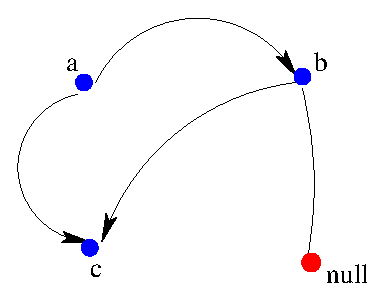
\includegraphics[totalheight=4.3 cm]{graph.eps}
        \end{center}
        \caption{Graph}
        \label{fig:graph}
\end{figure*}

We represent an oriented graph using $next/2$. The predicate $path/2$ succeeds
if there is a path between two nodes without cicles. We define that a node is
save if it is not connected to the node ``null'' (see Figure \ref{fig:graph}):

\begin{small}
\begin{verbatim}
next(a,b).
next(a,c).
next(b,c).
next(b,null).

path(X,X).
path(X,Y):- X=/=Y, next(X,Z),path(Z,Y).

save(X):- cneg(path(X,null)).
\end{verbatim}
\end{small}
So, we can ask for the nodes that are saved:
\begin{small}
\begin{verbatim}
?- save(X).

X=/=b,X=/=a,X=/=d ? ;

no
\end{verbatim}
\end{small}

%%%%%%%%%%%%%%%%%%%%%%%%%%%%%%%%%%%%%%%%%%%%%%%%%%%%%%%%%%%%%%%%%%
\subsection*{Bartak}

The following example was introduced by Bartak in \cite{Bartak}. In
http://kti. ms.mff.cuni.czJ ~bartak/html/negation.html there is a prototype
for constructive negation restricted to the case of finite computation trees.

\begin{small}
\begin{verbatim}
p(a,f(Z)):- t(Z).
p(f(Z),b):- t(Z).
t(c).
\end{verbatim}
\end{small}

Our implementation probide the following answers:

\begin{small}
\begin{verbatim}
?- cneg(p(X,Y)).

X=/=f(fA(_A)) ;

X=/=a,
Y=/=b ? ;

X = f(_A),
Y = b,
_A=/=c ? ;

Y=/=f(fA(_A)),
X=/=f(fA(_B)) ? ;

Y=/=b,Y=/=f(fA(_A)) ? ;

X = a,
Y = f(_A),
_A=/=c ? ;

no
\end{verbatim}
\end{small}

%%%%%%%%%%%%%%%%%%%%%%%%%%%%%%%%%%%%%%%%%%%%%%%%%%%%%%%%%%%%%%%%%%
\subsection*{Symmetric}

The next program computes symmetric (non-symmetric) terms of the signature
{f2/2,f1/1,o/0}. 
\begin{small}
\begin{verbatim}
symmetric(o). 
symmetric(f1(X)):- symmetric(X).
symmetric(f2(X,Y)):- mirror(X,Y).

mirror(o,o) .
mirror(f1(X),f1(Y)):- mirror(X,Y).
mirror(f2(X,Y),f2(Z,W)):- mirror(X,W),mirror(Y,Z).
\end{verbatim}
\end{small}

The query obtains the list of non symmetric terms:
\begin{small}
\begin{verbatim}
?- cneg(symmetric(Z)).

Z=/=f2(fA(_B),fA(_A)),Z=/=o,Z=/=f1(fA(_C)) ? ;

Z = f2(_A,_),
_A=/=f2(fA(_C),fA(_B)),_A=/=o,_A=/=f1(fA(_D)) ? ;

Z = f2(_A,_B),
_A=/=f1(fA(_E)),_A=/=o,
_B=/=f2(fA(_D),fA(_C)) ? ;

Z = f2(f2(_A,_),f2(_,_)),
_A=/=f2(fA(_C),fA(_B)),_A=/=o,_A=/=f1(fA(_D)) ? ;

Z = f2(f2(_D,_),f2(_,_A)),
_D=/=f1(fA(_E)),_D=/=o,
_A=/=f2(fA(_C),fA(_B)) ? ;

Z = f2(f2(f2(_A,_),_),f2(_,f2(_,_))),
_A=/=f2(fA(_C),fA(_B)),_A=/=o,_A=/=f1(fA(_D)) ? ;

...
\end{verbatim}
\end{small}
%%%%%%%%%%%%%%%%%%%%%%%%%%%%%%%%%%%%%%%%%%%%%%%%%%%%%%%%%%%%%%%%%%
\subsection*{Duplicates}

Definition of a predicate that checks or generates a list with duplicated
elements from \cite{Chan1}.
\begin{small}
\begin{verbatim}
member(X,[X|_]).
member(X,[_|Y]):- member(X,Y).

has_duplicates([X|Y]):- member(X,Y). 
has_duplicates([_|Y]):- has_duplicates(Y).

list_of_digits([ ]).
list_of_digits([X|Y]):- digit(X),list_of_digits(Y).

digit(l).
digit(2).
digit(3).
\end{verbatim}
\end{small}

The following question is an example of generate and test:
\begin{small}
\begin{verbatim}
?- L=[_,_,_], cneg(has_duplicates(L)), list_of_digits(L).

L = [l,2,3] ? ;

L = [l,3,2] ? ;

L = [2,l,3] ? ;

L = [2,3,l] ? ;

L = [3,l,2] ? ;

L = [3,2,l] ? ;

no
\end{verbatim}
\end{small}

%%%%%%%%%%%%%%%%%%%%%%%%%%%%%%%%%%%%%%%%%%%%%%%%%%%%%%%%%%%%%%%%%%
\subsection*{Disjoint}

The intuitive definition of disjoint lists includes a negation:
\begin{small}
\begin{verbatim}
disjoint([],_).
disjoint([X|L1],L2):- cneg(member(X,L2)), disjoint(L1,L2).
\end{verbatim}
\end{small}

With the above definition of $list_of_digits/1$ we can make the following
queries: 
\begin{small}
\begin{verbatim}
?-  disjoint([1,2,3],[X,Y]).

Y=/=3,Y=/=1,Y=/=2,
X=/=3,X=/=1,X=/=2 ? ;

no
?- list_of_digits([X,Y]),disjoint([1,2,3],[X,Y]).

no
?- list_of_digits([X,Y]),disjoint([1,2],[X,Y]).

X = 3,
Y = 3 ? ;

no
\end{verbatim}
\end{small}


\end{document}

